% Options for packages loaded elsewhere
\PassOptionsToPackage{unicode}{hyperref}
\PassOptionsToPackage{hyphens}{url}
%
\documentclass[
  12pt,
]{article}
\usepackage{amsmath,amssymb}
\usepackage{lmodern}
\usepackage{iftex}
\ifPDFTeX
  \usepackage[T1]{fontenc}
  \usepackage[utf8]{inputenc}
  \usepackage{textcomp} % provide euro and other symbols
\else % if luatex or xetex
  \usepackage{unicode-math}
  \defaultfontfeatures{Scale=MatchLowercase}
  \defaultfontfeatures[\rmfamily]{Ligatures=TeX,Scale=1}
\fi
% Use upquote if available, for straight quotes in verbatim environments
\IfFileExists{upquote.sty}{\usepackage{upquote}}{}
\IfFileExists{microtype.sty}{% use microtype if available
  \usepackage[]{microtype}
  \UseMicrotypeSet[protrusion]{basicmath} % disable protrusion for tt fonts
}{}
\makeatletter
\@ifundefined{KOMAClassName}{% if non-KOMA class
  \IfFileExists{parskip.sty}{%
    \usepackage{parskip}
  }{% else
    \setlength{\parindent}{0pt}
    \setlength{\parskip}{6pt plus 2pt minus 1pt}}
}{% if KOMA class
  \KOMAoptions{parskip=half}}
\makeatother
\usepackage{xcolor}
\IfFileExists{xurl.sty}{\usepackage{xurl}}{} % add URL line breaks if available
\IfFileExists{bookmark.sty}{\usepackage{bookmark}}{\usepackage{hyperref}}
\hypersetup{
  hidelinks,
  pdfcreator={LaTeX via pandoc}}
\urlstyle{same} % disable monospaced font for URLs
\usepackage[margin=1in]{geometry}
\usepackage{longtable,booktabs,array}
\usepackage{calc} % for calculating minipage widths
% Correct order of tables after \paragraph or \subparagraph
\usepackage{etoolbox}
\makeatletter
\patchcmd\longtable{\par}{\if@noskipsec\mbox{}\fi\par}{}{}
\makeatother
% Allow footnotes in longtable head/foot
\IfFileExists{footnotehyper.sty}{\usepackage{footnotehyper}}{\usepackage{footnote}}
\makesavenoteenv{longtable}
\usepackage{graphicx}
\makeatletter
\def\maxwidth{\ifdim\Gin@nat@width>\linewidth\linewidth\else\Gin@nat@width\fi}
\def\maxheight{\ifdim\Gin@nat@height>\textheight\textheight\else\Gin@nat@height\fi}
\makeatother
% Scale images if necessary, so that they will not overflow the page
% margins by default, and it is still possible to overwrite the defaults
% using explicit options in \includegraphics[width, height, ...]{}
\setkeys{Gin}{width=\maxwidth,height=\maxheight,keepaspectratio}
% Set default figure placement to htbp
\makeatletter
\def\fps@figure{htbp}
\makeatother
\setlength{\emergencystretch}{3em} % prevent overfull lines
\providecommand{\tightlist}{%
  \setlength{\itemsep}{0pt}\setlength{\parskip}{0pt}}
\setcounter{secnumdepth}{-\maxdimen} % remove section numbering
\ifLuaTeX
  \usepackage{selnolig}  % disable illegal ligatures
\fi

\author{}
\date{}

\begin{document}

\begin{titlepage}
\centering
\vspace*{0.85in}
{\Large\bfseries UNIVERSITY OF NEW HAMPSHIRE\par}
\vspace{0.35in}
\rule{0.58\textwidth}{0.4pt}\par
\vspace{0.85in}
{\LARGE\bfseries Monte Carlo Assessment of Two-Sided $8\,\mathrm{MeV}$ Electron Irradiation of Cryogenic ND$_3$ for Polarized Target Preparation\par}
\vspace{0.55in}
{\large Journal Manuscript\par}
\vspace{0.55in}
{\large Samuel Takwirira\par}
\vspace{0.25in}
{UNH DNP Group\par}
{University of New Hampshire\par}
{Jefferson Lab Target Group Collaboration\par}
\vfill
{May 2026\par}
\end{titlepage}

\hypertarget{abstract}{%
\section{Abstract}\label{abstract}}

Polarized solid targets based on ammonia require a controlled density of
radiation-induced paramagnetic centers to support dynamic nuclear
polarization (DNP) {[}3,4{]}. For deuterated ammonia (ND3), the
irradiation procedure must be evaluated not only by the incident
electron fluence, but also by the depth dependence of deposited dose,
target-volume coverage, secondary radiation environment, and cryogenic
heat load. A TOPAS/Geant4 Monte Carlo model {[}1,2{]} was developed to
assess an \(8\,\mathrm{MeV}\) electron irradiation protocol for a packed
cryogenic ND3 target at the Jefferson Lab Upgraded Injector Test
Facility (UITF). The model includes the beam-spreading aluminum window,
cryostat windows, liquid-helium bath, target-holder proxy, packed ND3
target volume, front and back electron sources, depth-dose scorers,
radial-dose scorers, R-Z dose maps, fluence scorers, spectral
diagnostics, and total energy-deposition checks.

Because the target length is \(6.5\,\mathrm{cm}\) {[}7{]}, the
simulation treats the irradiation as a two-sided protocol: one run
irradiates the upstream face and a second run irradiates the downstream
face. The back-side dose field is oriented into the same target
coordinate system before summation. This distinction is essential: front
and back exposures are sequential and must not be interpreted as
simultaneous heat loads. The available completed front/back analysis,
normalized per primary and scaled to proposal beam currents, gives a
cold \(1\,\mu\mathrm{A}\) delivered fluence of
\(4.97 \times 10^{15}\,\mathrm{e}^{-}\,\mathrm{cm}^{-2}\) per side and
\(9.94 \times 10^{15}\,\mathrm{e}^{-}\,\mathrm{cm}^{-2}\) for the
two-sided exposure. The mean cold cumulative dose is
\(1.32 \times 10^{6}\,\mathrm{Gy}\) per side and
\(2.63 \times 10^{6}\,\mathrm{Gy}\) after front/back exposure, with an
estimated deposited power of \(0.064\,\mathrm{W}\) per active side. The
warm \(10\,\mu\mathrm{A}\) case gives
\(9.97 \times 10^{16}\,\mathrm{e}^{-}\,\mathrm{cm}^{-2}\) per side,
\(5.29 \times 10^{7}\,\mathrm{Gy}\) mean two-sided cumulative dose, and
\(0.644\,\mathrm{W}\) per active side.

The simulation supports a physically traceable two-sided irradiation
protocol for polarized-target material preparation. It directly predicts
electron/photon transport, dose, fluence, energy deposition, and heat
load. It does not directly predict radical species, radical survival,
annealing behavior, ESR spectra, or final DNP polarization; those
material-response quantities require experimental benchmarking.

\textbf{Keywords:} polarized target, dynamic nuclear polarization, ND3,
ammonia irradiation, electron irradiation, TOPAS, Geant4, dose, fluence,
LET, cryogenic heat load.

\hypertarget{introduction}{%
\section{1. Introduction}\label{introduction}}

Solid ammonia targets are central to polarized fixed-target experiments
because they combine high achievable nuclear polarization, comparatively
favorable dilution factors, and strong radiation resistance under
experimental beam conditions {[}3,4{]}. In these materials, DNP is
enabled by unpaired electron spins associated with radiation-induced
paramagnetic centers {[}4,5{]}. The irradiation step is therefore part
of the polarized-target preparation physics, not merely an activation or
handling procedure. It establishes the defect population that later
couples to the nuclear spin system through microwave-driven polarization
transfer and spin diffusion.

For ND3, the irradiation requirements are especially important because
the deuteron polarization performance depends sensitively on the type,
density, and spatial distribution of the radiation-induced centers
{[}5,6{]}. A useful irradiation protocol must deliver sufficient
ionization dose to the material while avoiding excessive thermal load
and gross nonuniformity. The relevant observables are therefore not only
total incident charge or beam time; they include electron fluence,
deposited dose, dose uniformity, depth dependence, energy deposition
rate, secondary radiation, and LET-like track-structure proxies.

This work presents a Monte Carlo assessment {[}1,2{]} of a two-sided
\(8\,\mathrm{MeV}\) electron irradiation concept for cryogenic packed
ND3. The simulation is designed around the specific polarized-target
question: whether the beamline and target geometry can plausibly create
a proposal-scale radiation field throughout the sample volume while
maintaining a credible cold-operation heat load. Here we show that the
target length and electron range require a two-sided irradiation
interpretation, and we quantify the resulting dose, fluence, spectral
diagnostics, and per-side heat-load scale for the proposed operating
points.

\hypertarget{methods-and-analysis-framework}{%
\section{2. Methods and Analysis
Framework}\label{methods-and-analysis-framework}}

\hypertarget{fluence}{%
\subsection{2.1 Fluence}\label{fluence}}

Fluence, \(\Phi\), is the number of particles incident on or crossing a
unit area, commonly expressed here as
\(\mathrm{e}^{-}\,\mathrm{cm}^{-2}\). In polarized ammonia preparation,
fluence is a practical irradiation-control variable because facilities
often prescribe an electron dose target as an integrated number of
electrons per unit sample area. Fluence is not the same as absorbed
dose: two beams with the same fluence can deposit different energy
depending on energy, material composition, geometry, and scattering. In
this work, fluence is used to compare the simulation to the proposal
targets {[}7{]} of
\(5.0 \times 10^{15}\,\mathrm{e}^{-}\,\mathrm{cm}^{-2}\) per side for
cold irradiation and
\(1.0 \times 10^{17}\,\mathrm{e}^{-}\,\mathrm{cm}^{-2}\) per side for
warm irradiation.

\hypertarget{absorbed-dose}{%
\subsection{2.2 Absorbed Dose}\label{absorbed-dose}}

Absorbed dose, \(D\), is the energy deposited per unit mass of material,
measured in gray {[}1{]}, where
\(1\,\mathrm{Gy} = 1\,\mathrm{J}\,\mathrm{kg}^{-1}\). For irradiated
polarized targets, dose is relevant because radical production is driven
by deposited ionization energy. The spatial distribution of dose
matters: a target batch with large underdosed regions may have
insufficient paramagnetic-center density, while localized overdosed
regions can promote damage, heating, or nonuniform material response.

\hypertarget{linear-energy-transfer-and-let-like-proxies}{%
\subsection{2.3 Linear Energy Transfer and LET-like
Proxies}\label{linear-energy-transfer-and-let-like-proxies}}

Linear energy transfer (LET) describes energy deposition per unit track
length, often reported in \(\mathrm{keV}/\mu\mathrm{m}\). LET is
relevant because the local ionization density can influence radical
formation, recombination probability, and the balance of paramagnetic
species. For low-energy electron transport in this TOPAS setup, a direct
generic electron LET scorer is not treated as the primary observable.
Instead, LET-like behavior is inferred in post-processing from deposited
energy and fluence trends. These quantities should be used as
track-structure indicators, not as direct chemical predictions.

\hypertarget{heat-load}{%
\subsection{2.4 Heat Load}\label{heat-load}}

At cryogenic temperature, deposited energy becomes a thermal-design
constraint. The quantity of interest is deposited power during one
active irradiation side. The front and back irradiations are sequential;
therefore, the instantaneous heat load is the per-side load, not the sum
of both sides. This distinction is central for assessing whether the
cold irradiation case is compatible with the available refrigeration
power.

\hypertarget{spectral-and-secondary-radiation-diagnostics}{%
\subsection{2.5 Spectral and Secondary Radiation
Diagnostics}\label{spectral-and-secondary-radiation-diagnostics}}

The entrance electron spectrum verifies that the target sees the
intended beam after upstream materials. Exit bremsstrahlung and gamma
fluence contextualize shielding and background, but they are not primary
DNP observables. They are included because a publishable irradiation
study must demonstrate that the beam transport and secondary radiation
environment are understood.

\hypertarget{monte-carlo-transport}{%
\subsection{2.6 Monte Carlo Transport}\label{monte-carlo-transport}}

The simulation was implemented in TOPAS as a front end to Geant4
particle transport {[}1,2{]}. TOPAS is used here as a general Monte
Carlo research tool for electron and photon transport in a
polarized-target irradiation geometry. The physics emphasis is
electromagnetic energy deposition in cryogenic target material and
surrounding beamline components.

\hypertarget{beam-and-geometry}{%
\subsection{2.7 Beam and Geometry}\label{beam-and-geometry}}

The incident beam is an \(8\,\mathrm{MeV}\) electron beam rastered over
a circular field of \(14.3\,\mathrm{mm}\) radius, corresponding to
approximately \(6.42\,\mathrm{cm}^{2}\) interaction area {[}7{]}. The
model includes a beam-spreading aluminum element, aluminum cryostat
entrance and exit windows, a liquid-helium cold bath, a target-holder
proxy, a packed ND3 target region, and downstream scoring and dump
regions.

The target is modeled as a \(6.5\,\mathrm{cm}\) long cylindrical packed
ND3 volume with radius \(1.42\,\mathrm{cm}\) {[}7{]}. The proposal-scale
batch mass is \(250\,\mathrm{mg}\) {[}7{]}. Thus, the primary target
material is represented as a bulk-average packed material distributed
over the holder volume. This choice preserves the batch-level mass and
heat-load normalization. A separate single-bead branch exists for
microdosimetry checks, but the batch-level results are reported from the
packed target volume.

\hypertarget{two-sided-irradiation-protocol}{%
\subsection{2.8 Two-Sided Irradiation
Protocol}\label{two-sided-irradiation-protocol}}

The \(8\,\mathrm{MeV}\) electron range makes a one-sided exposure
inadequate for representing the full \(6.5\,\mathrm{cm}\) target length.
The protocol is therefore represented by two separate simulations:

\begin{enumerate}
\def\labelenumi{\arabic{enumi}.}
\tightlist
\item
  Front-side irradiation: the beam enters the upstream target face.
\item
  Back-side irradiation: the beam enters the downstream target face.
\end{enumerate}

The combined target-coordinate dose is:

\[
D_{\mathrm{FB}}(z) = D_{\mathrm{front}}(z) + D_{\mathrm{back,oriented}}(z),
\]

where \(D_{\mathrm{back,oriented}}(z)\) is the back-side dose profile
expressed in the same coordinate system as the front-side result. This
is a cumulative two-exposure dose. It is not a simultaneous two-beam
heat-load condition.

\hypertarget{scorers}{%
\subsection{2.9 Scorers}\label{scorers}}

The principal scored quantities are:

\begin{itemize}
\tightlist
\item
  depth dose in packed ND3;
\item
  R-Z dose map in packed ND3;
\item
  radial dose uniformity;
\item
  target energy deposition;
\item
  fluence versus depth;
\item
  entrance and exit target fluence;
\item
  entrance electron energy spectrum;
\item
  exit photon and bremsstrahlung spectra;
\item
  target and cryogenic-bath energy-deposition checks;
\item
  upstream backscatter.
\end{itemize}

These scorers form a validation chain: beam transport, target entry,
longitudinal dose, radial coverage, secondary radiation, and deposited
power are all checked before interpreting the irradiation as suitable
for polarized-target preparation.

\hypertarget{normalization}{%
\subsection{2.10 Normalization}\label{normalization}}

TOPAS scorer sums are divided by the number of simulated primary
electron histories to obtain per-primary values. Physical scaling to
beam current uses:

\[
\dot{D}(z) = D_{\mathrm{primary}}(z)\frac{I}{e},
\]

where \(I\) is beam current and \(e = 1.602176634 \times 10^{-19}\) C.
Cumulative dose is obtained by multiplying the dose rate by irradiation
time per side. Deposited power is computed from total deposited energy
per primary multiplied by the electron rate \(I/e\).

The operating points used for physical interpretation are taken from the
proposal conditions {[}7{]}:

\begin{itemize}
\tightlist
\item
  cold irradiation: \(1\,\mu\mathrm{A}\), 1.42 hours per side;
\item
  warm irradiation: \(10\,\mu\mathrm{A}\), 2.85 hours per side.
\end{itemize}

\hypertarget{results-and-analysis}{%
\section{3. Results and Analysis}\label{results-and-analysis}}

\hypertarget{front-and-back-depth-dose-profiles}{%
\subsection{3.1 Front and Back Depth-Dose
Profiles}\label{front-and-back-depth-dose-profiles}}

The front-only depth-dose profile is range-limited across the
\(6.5\,\mathrm{cm}\) target length. The downstream/back exposure
complements the front exposure when expressed in target coordinates.
This is the central physics justification for two-sided irradiation.

\begin{figure}
\centering
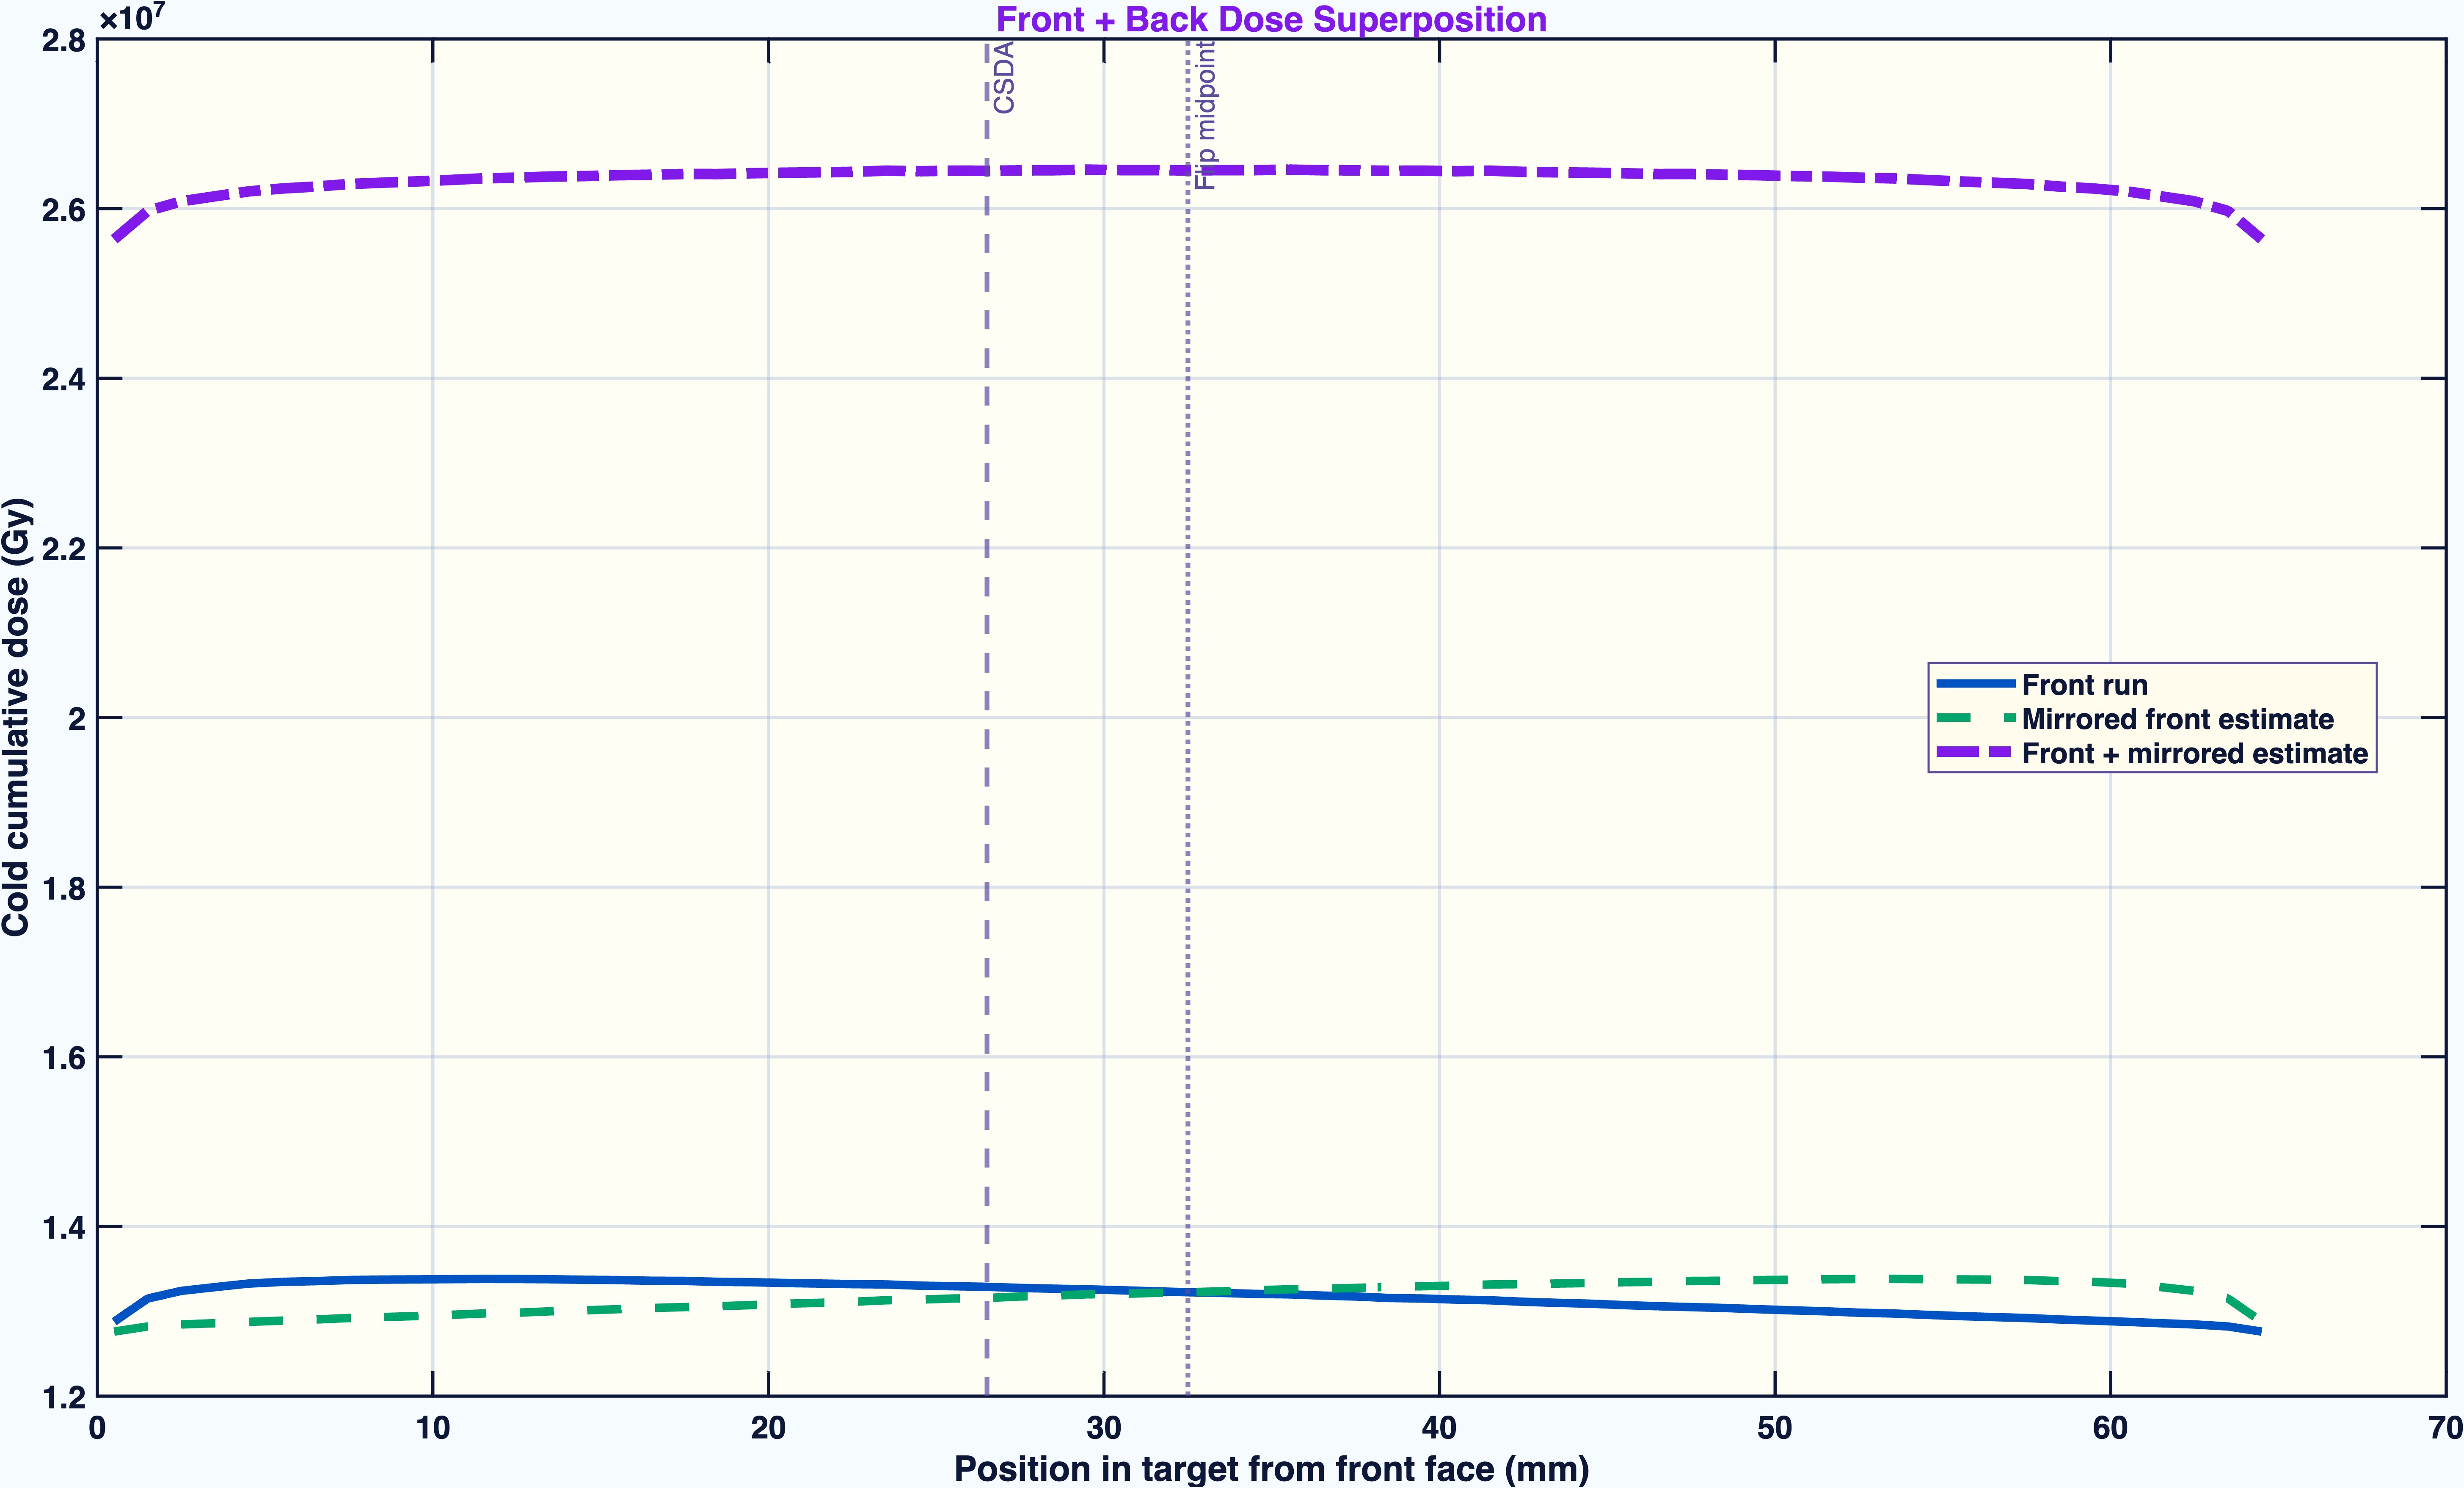
\includegraphics{./figures_matlab/pptx_deck_assets/01_front_back_superimposed_cold_dose.png}
\caption{Figure 1. Front, back, and combined cold cumulative dose
profiles.}
\end{figure}

\textbf{Figure 1.} Front-side, back-side, and front-plus-back cold
cumulative dose profiles. The figure demonstrates why a one-sided
\(8\,\mathrm{MeV}\) exposure is not a sufficient representation of the
target-volume dose. The combined curve is the cumulative dose from two
sequential exposures.

\hypertarget{combined-cold-dose-field}{%
\subsection{3.2 Combined Cold Dose
Field}\label{combined-cold-dose-field}}

The combined front/back curve is the proposal-relevant target-coordinate
dose field. For the cold \(1\,\mu\mathrm{A}\) case, the mean cumulative
dose is \(1.32 \times 10^{6}\,\mathrm{Gy}\) per side and
\(2.63 \times 10^{6}\,\mathrm{Gy}\) after front/back exposure.

\begin{figure}
\centering
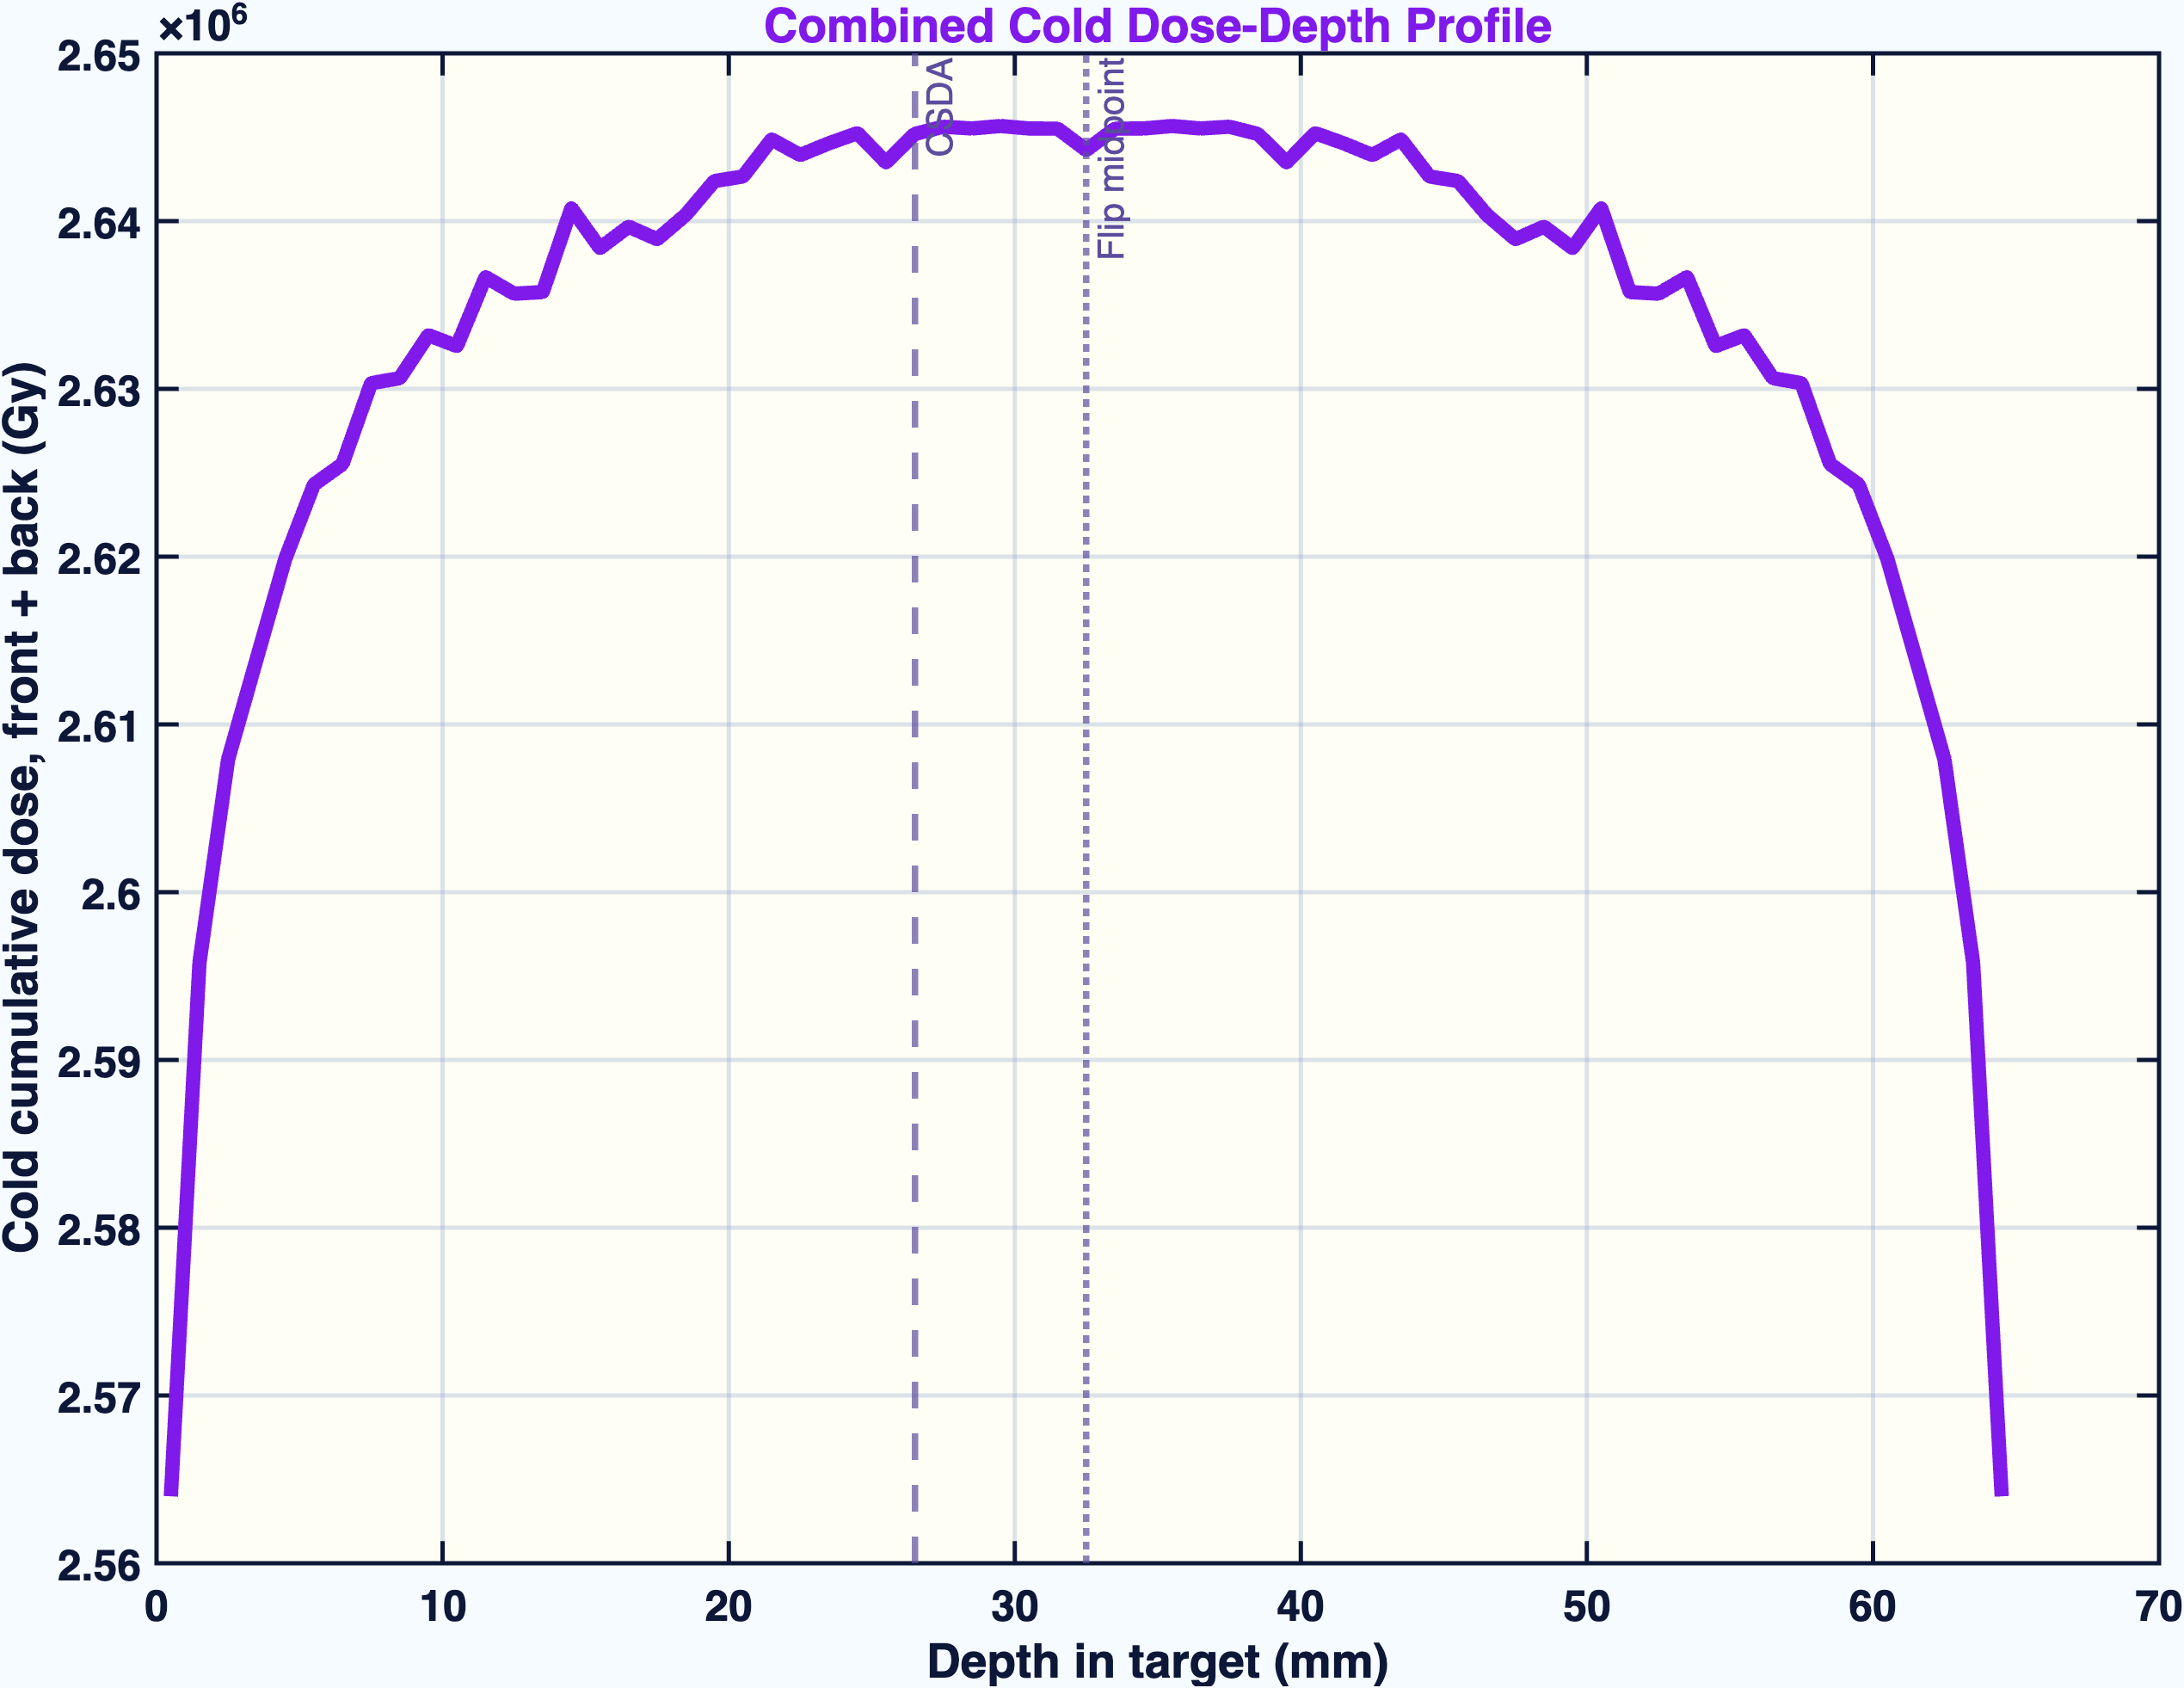
\includegraphics{./figures_matlab/pptx_deck_assets/02_combined_cold_dose_depth.png}
\caption{Figure 2. Combined cold dose-depth profile.}
\end{figure}

\textbf{Figure 2.} Combined cold dose-depth profile for the two-sided
irradiation protocol. This curve is the primary depth-dose result for
cold ND3 irradiation.

\hypertarget{r-z-dose-map-and-target-coverage}{%
\subsection{3.3 R-Z Dose Map and Target
Coverage}\label{r-z-dose-map-and-target-coverage}}

The R-Z map tests whether the rastered beam covers the target radius and
whether the longitudinal dose field has obvious hot or cold regions. For
polarized-target preparation, this is a material-quality question: large
spatial nonuniformity would imply nonuniform radical density and
potentially nonuniform DNP behavior across the batch.

\begin{figure}
\centering
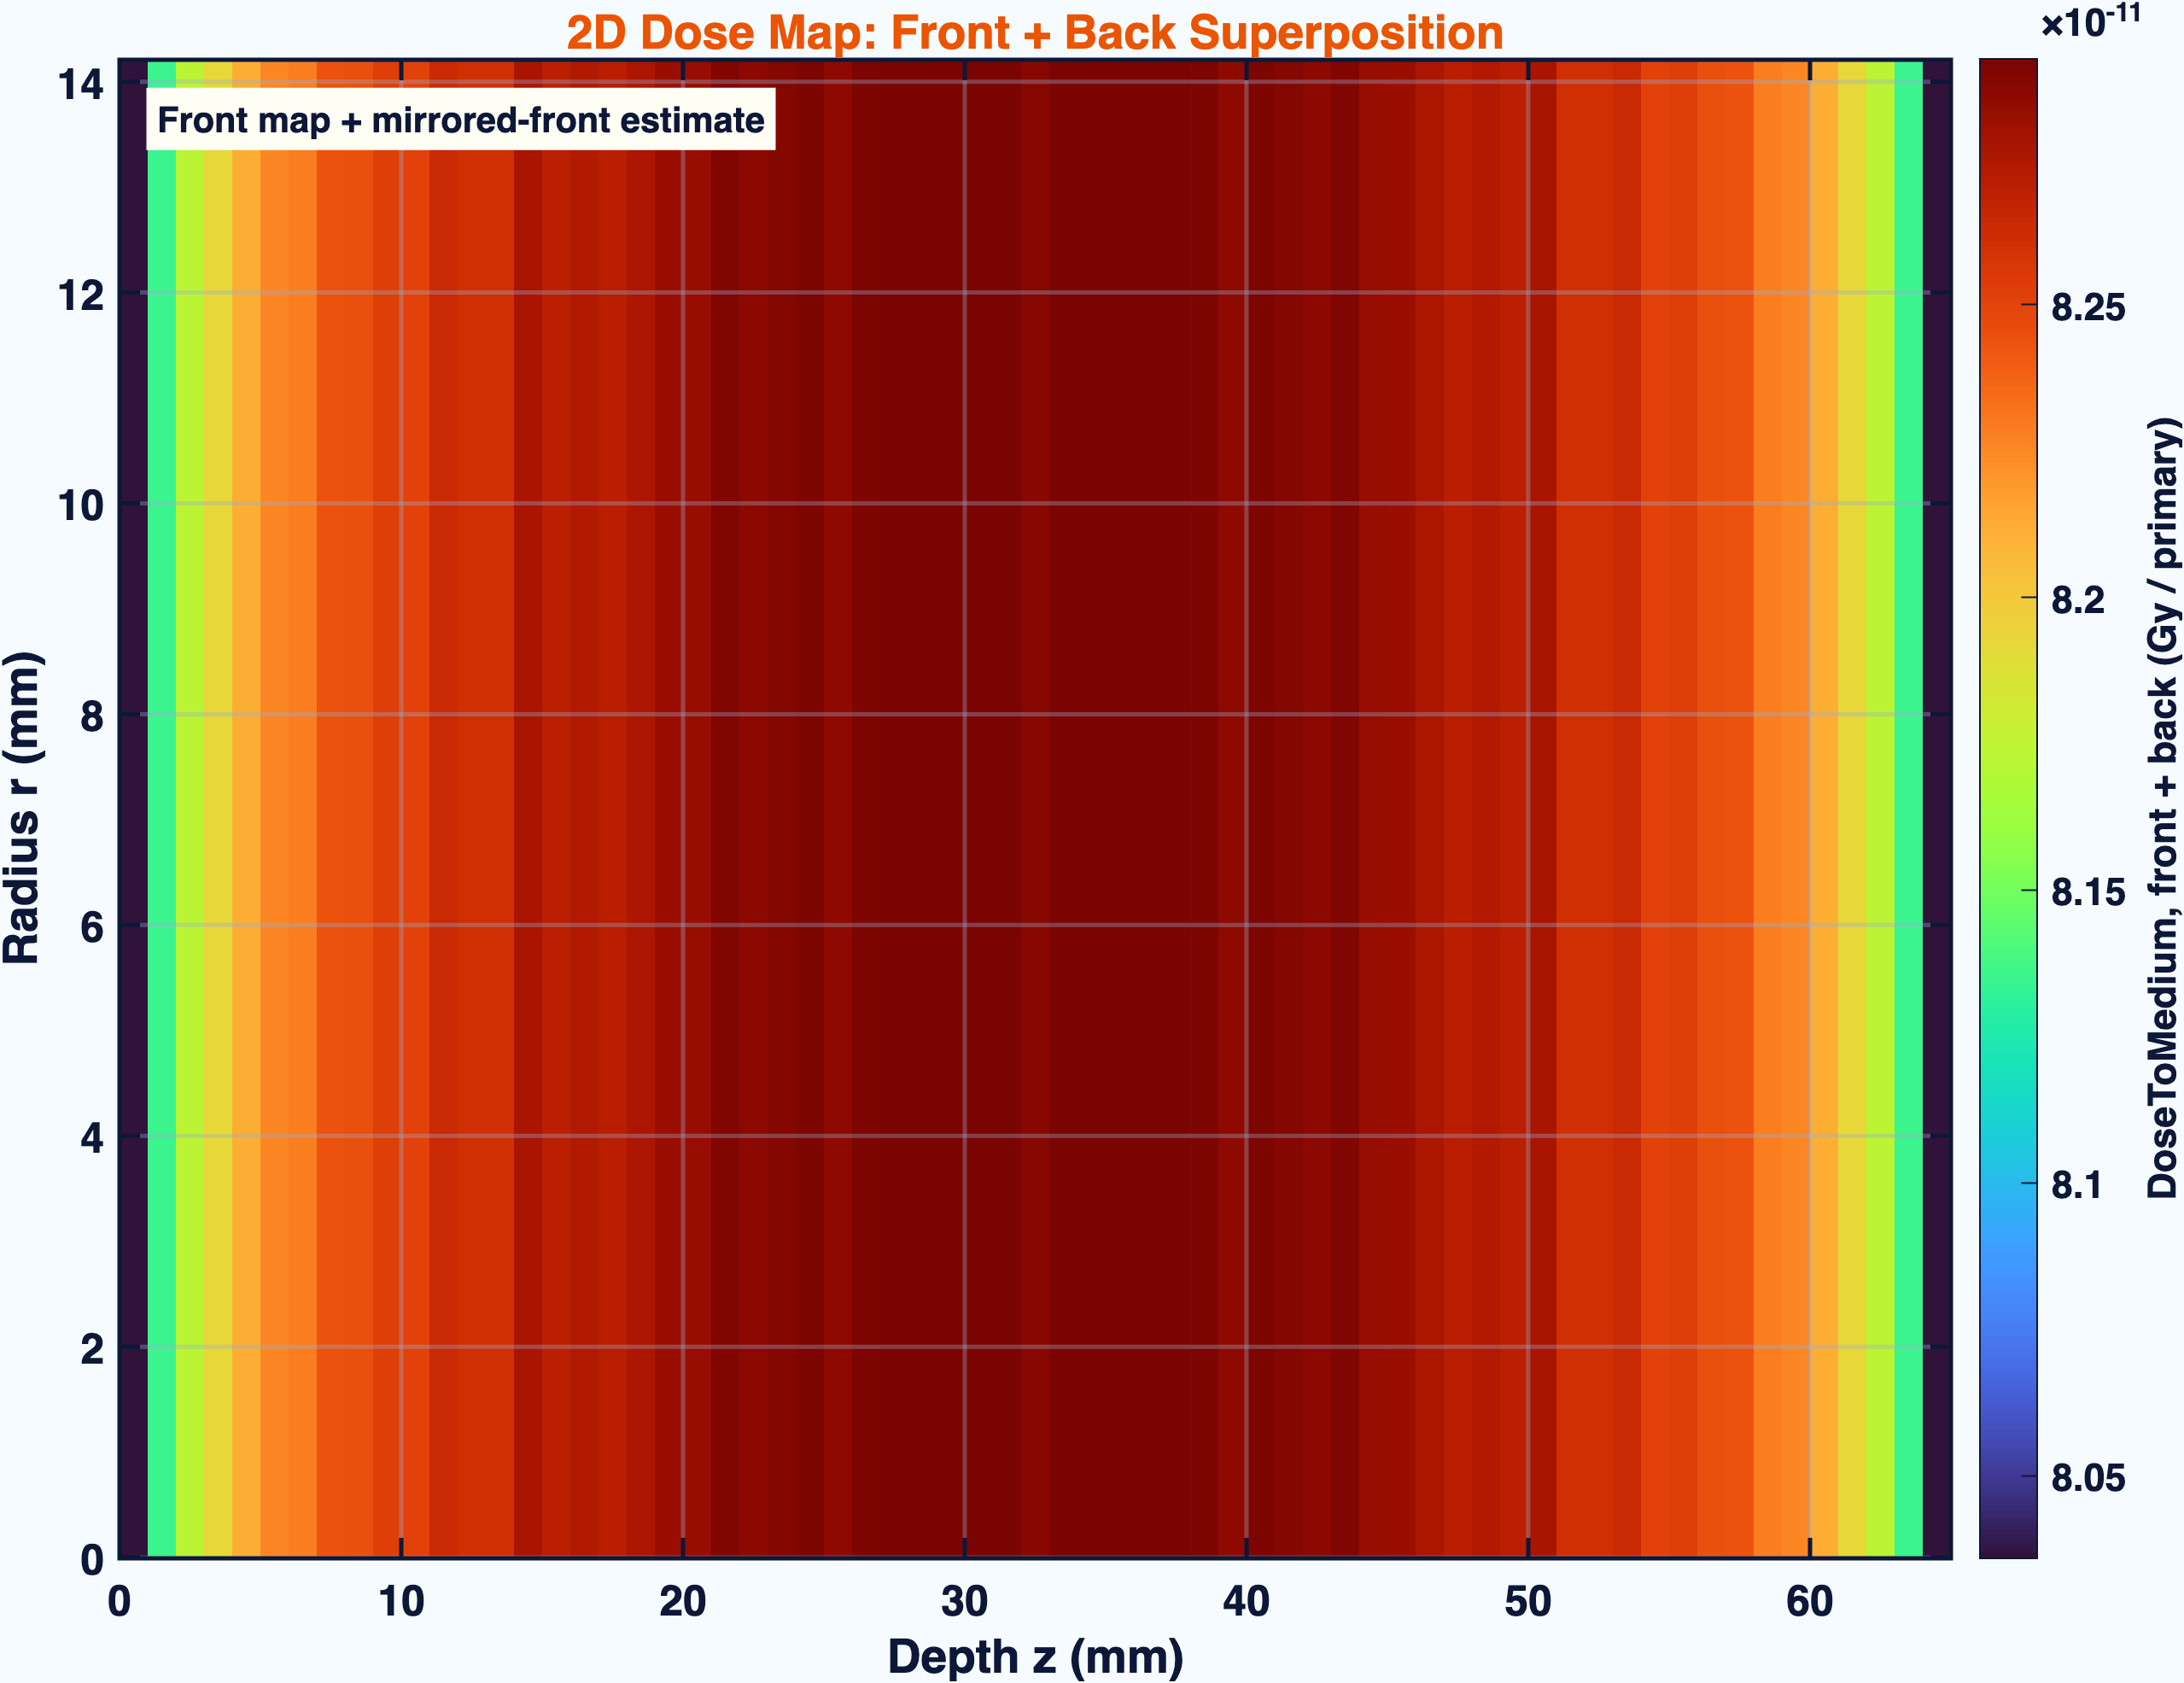
\includegraphics{./figures_matlab/pptx_deck_assets/03_2d_dose_map_superimposed.png}
\caption{Figure 3. Front-plus-back R-Z dose map.}
\end{figure}

\textbf{Figure 3.} R-Z dose map for the front-plus-back irradiation. The
map provides the spatial check that the target volume, rather than only
the central beam axis, is being evaluated.

\hypertarget{electron-fluence-through-the-target}{%
\subsection{3.4 Electron Fluence Through the
Target}\label{electron-fluence-through-the-target}}

Fluence versus depth is a beam-transport diagnostic and a
polarized-target irradiation metric. In this context, it shows how the
electron population evolves through the target and supports the
comparison between simulated irradiation and proposal fluence targets.

\begin{figure}
\centering
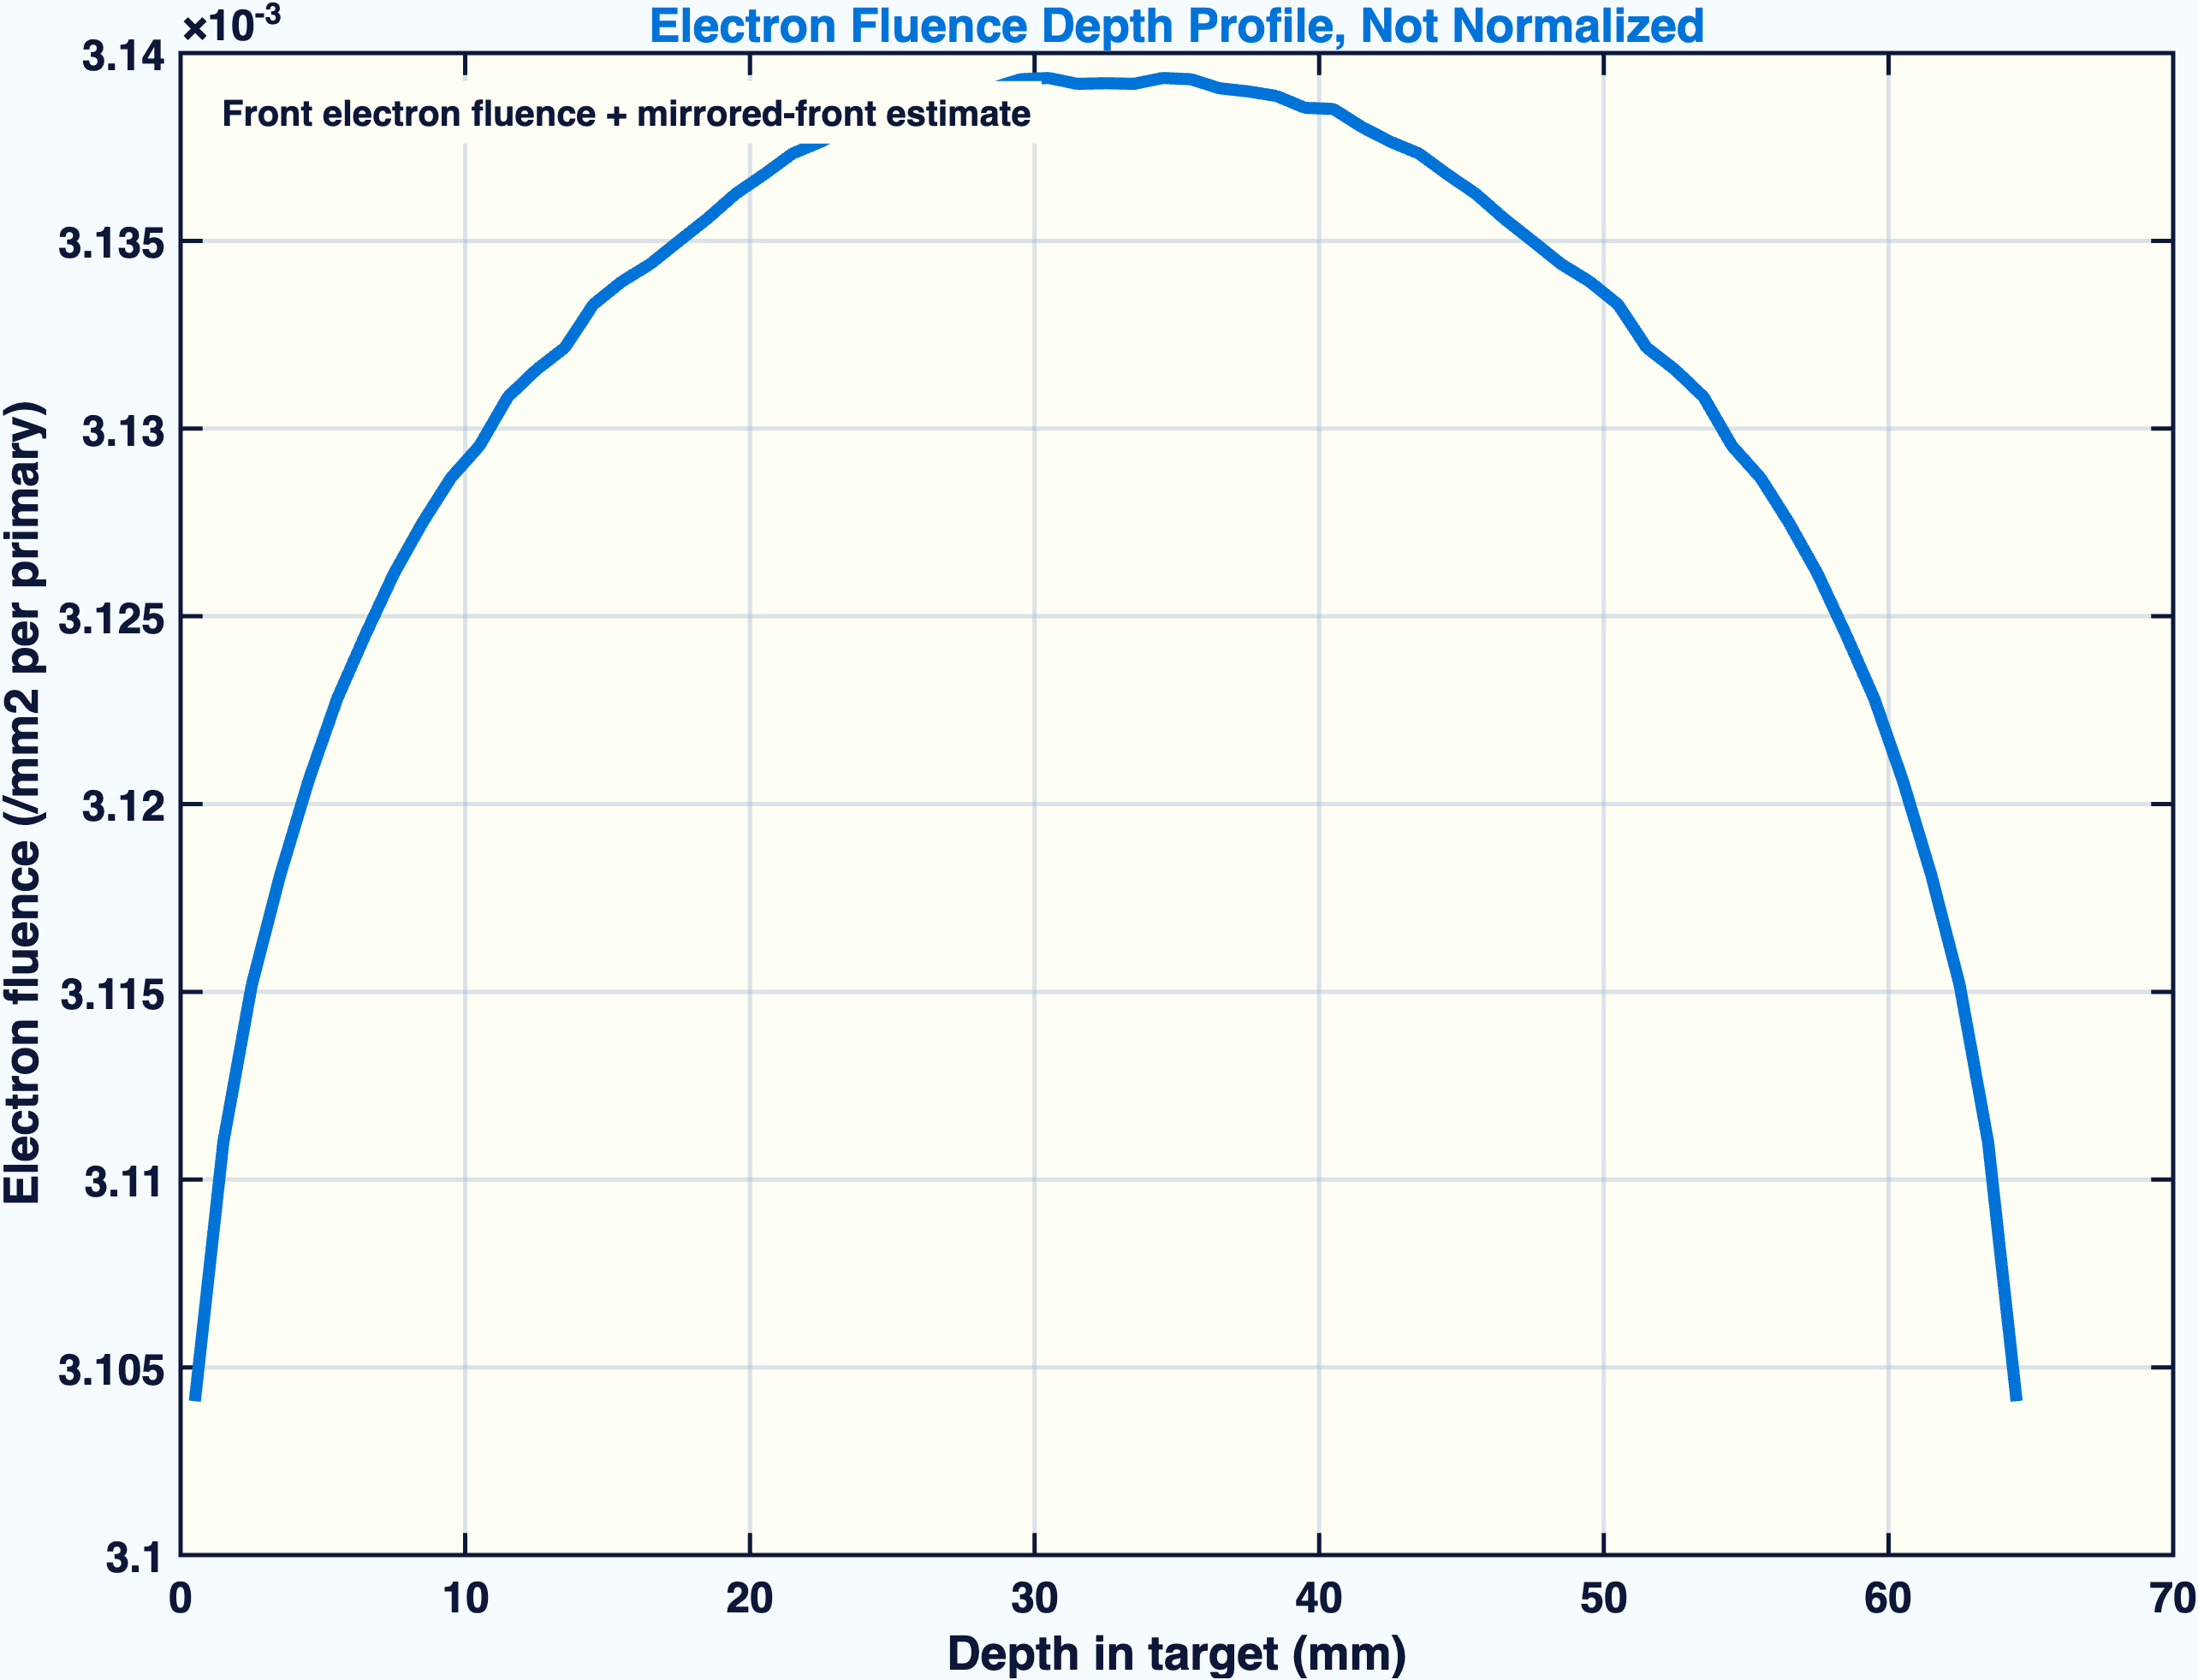
\includegraphics{./figures_matlab/pptx_deck_assets/04_electron_fluence_depth_unnormalized.png}
\caption{Figure 4. Electron fluence depth diagnostic.}
\end{figure}

\textbf{Figure 4.} Electron fluence versus target depth. Fluence is
reported as the number of electrons crossing unit area and is used to
connect Monte Carlo transport to the integrated electron exposure
prescribed for target-material irradiation.

\hypertarget{radial-dose-uniformity}{%
\subsection{3.5 Radial Dose Uniformity}\label{radial-dose-uniformity}}

Radial uniformity determines whether the rastered field gives a broad
irradiation over the sample area. This is important because the radical
inventory should be as uniform as practical across the batch, especially
if material is later loaded into polarized target cells where local
polarization and radiation resistance matter.

\begin{figure}
\centering
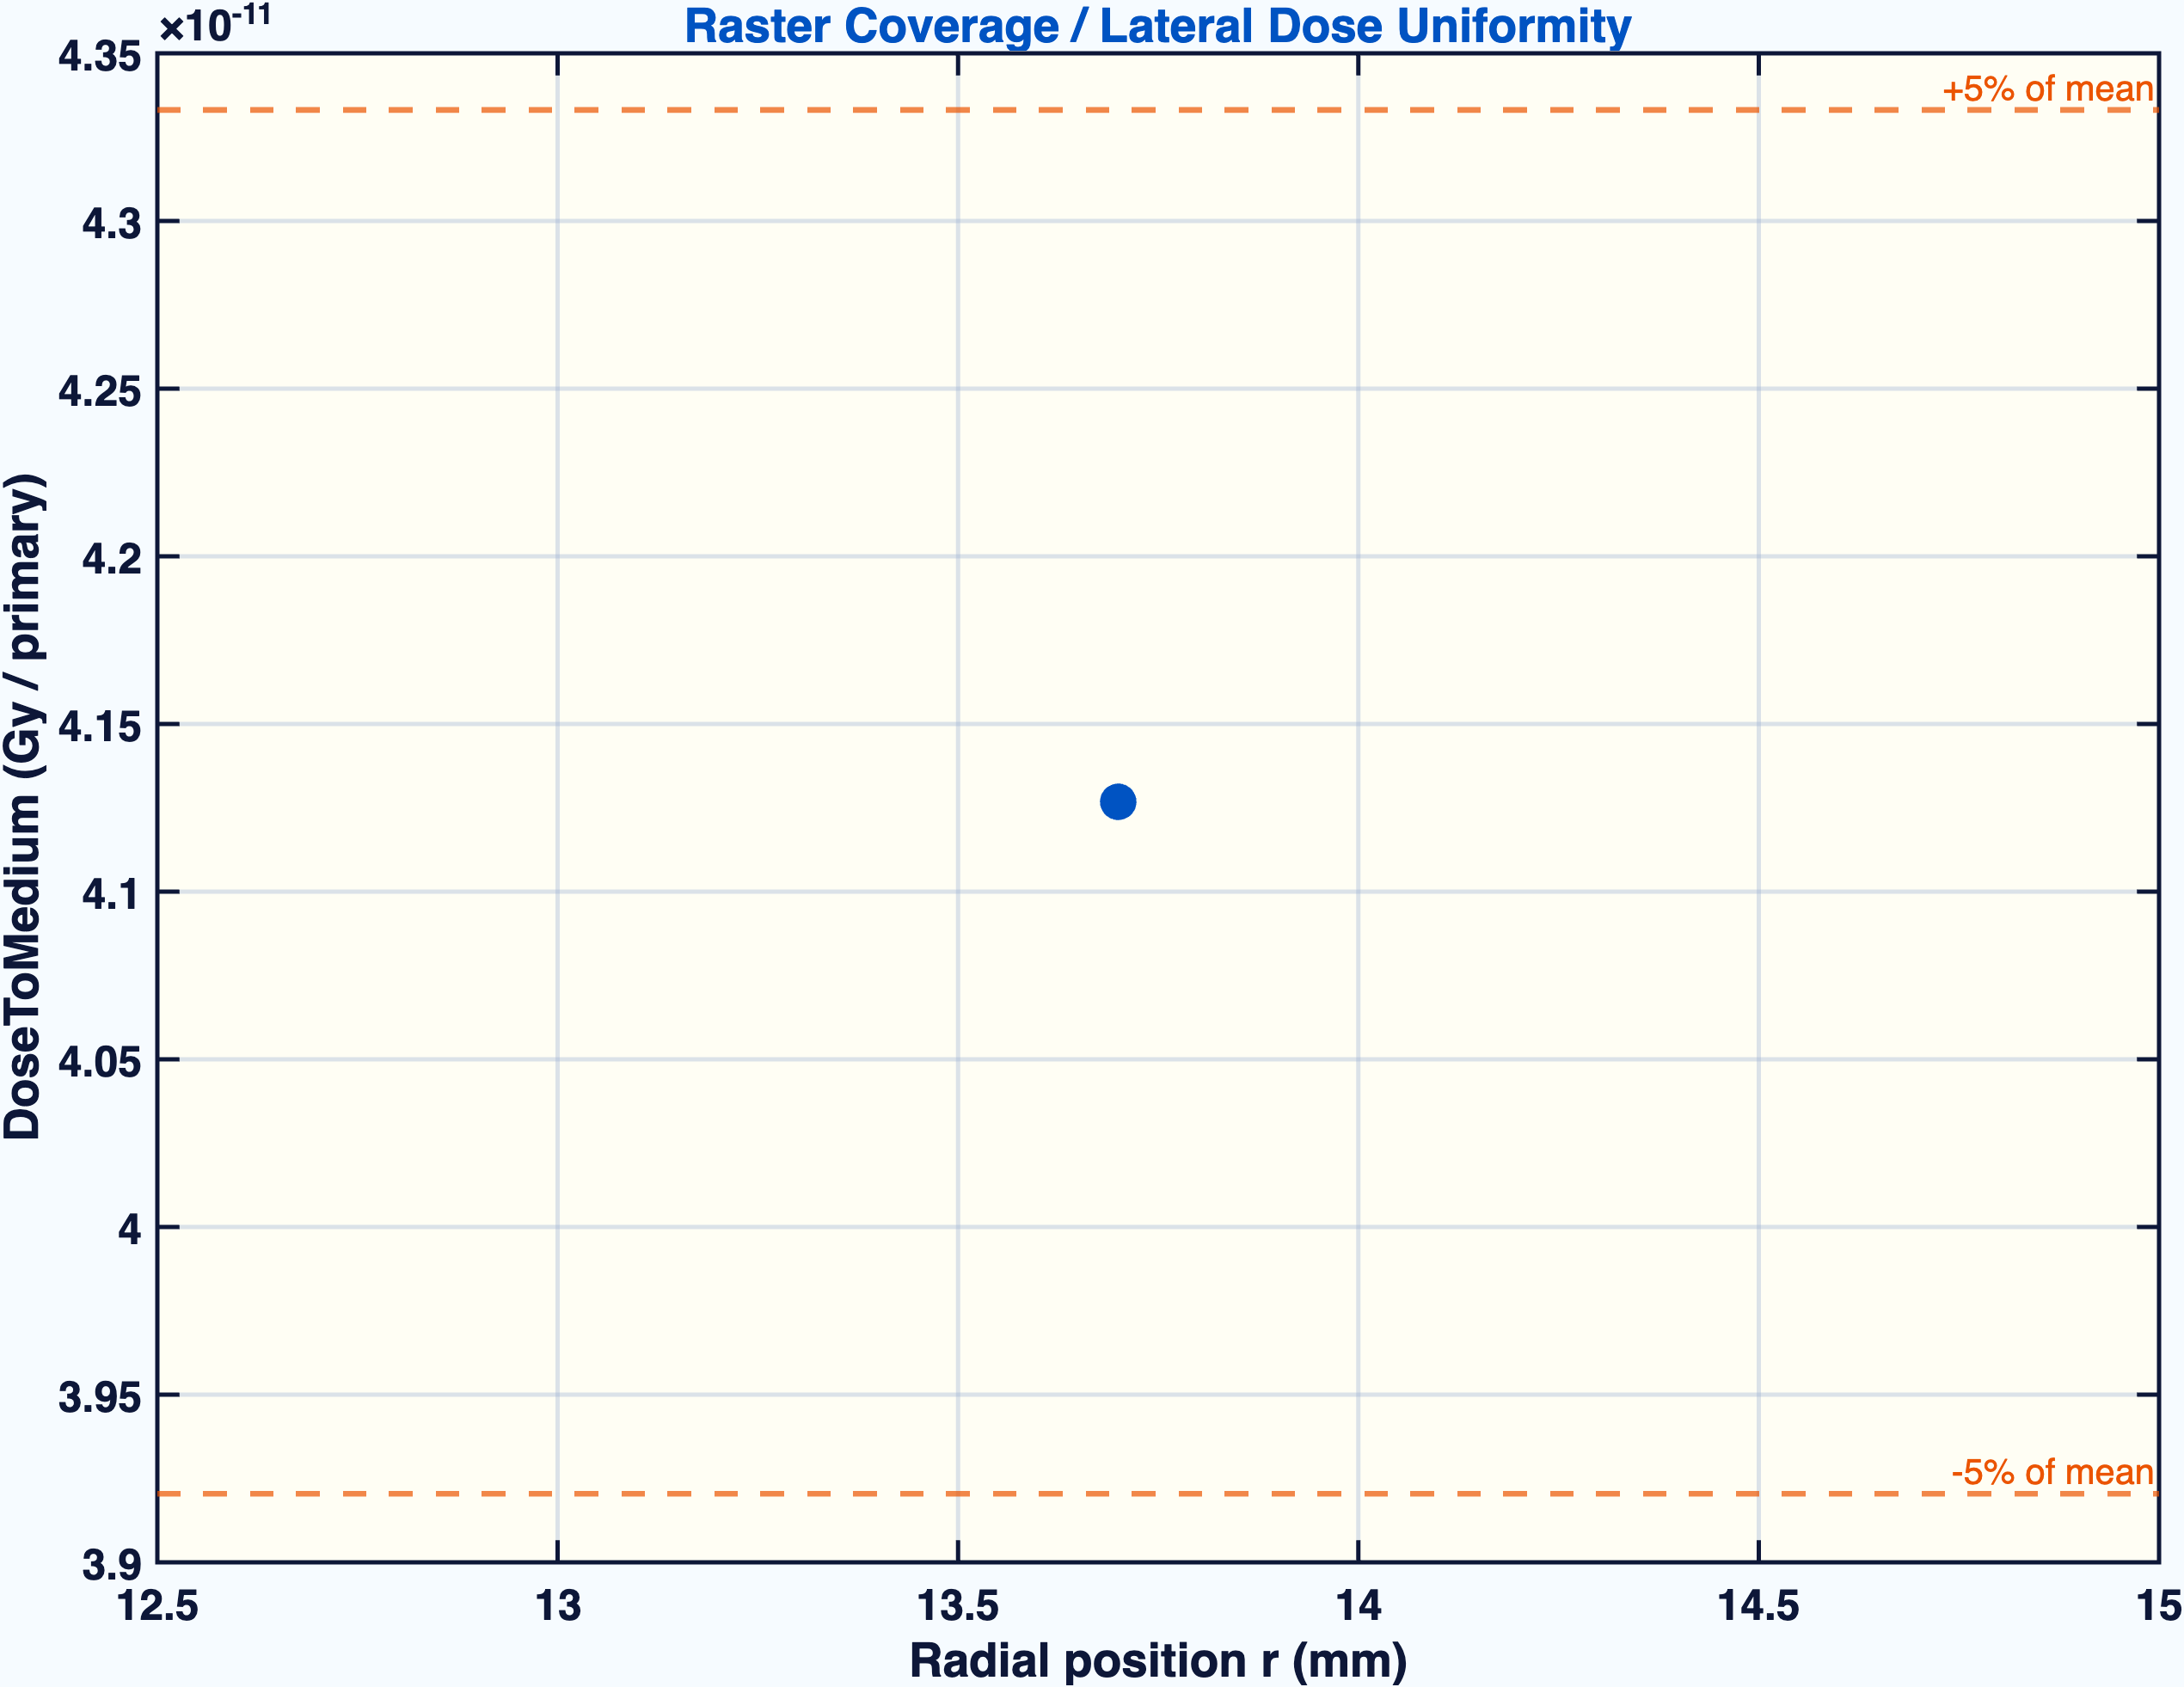
\includegraphics{./figures_matlab/pptx_deck_assets/06_lateral_dose_uniformity_raw.png}
\caption{Figure 5. Lateral dose uniformity.}
\end{figure}

\textbf{Figure 5.} Lateral dose uniformity across the target radius. The
figure checks whether the simulated raster provides broad target
coverage rather than a narrow pencil-beam exposure.

\hypertarget{spectral-diagnostics}{%
\subsection{3.6 Spectral Diagnostics}\label{spectral-diagnostics}}

The entrance spectrum verifies the electron energy reaching the target.
The photon spectrum at exit quantifies the bremsstrahlung environment.
For polarized targets, the entrance electron spectrum is relevant to
dose and radical production, while the photon spectrum is mainly a
shielding and background diagnostic.

\begin{figure}
\centering
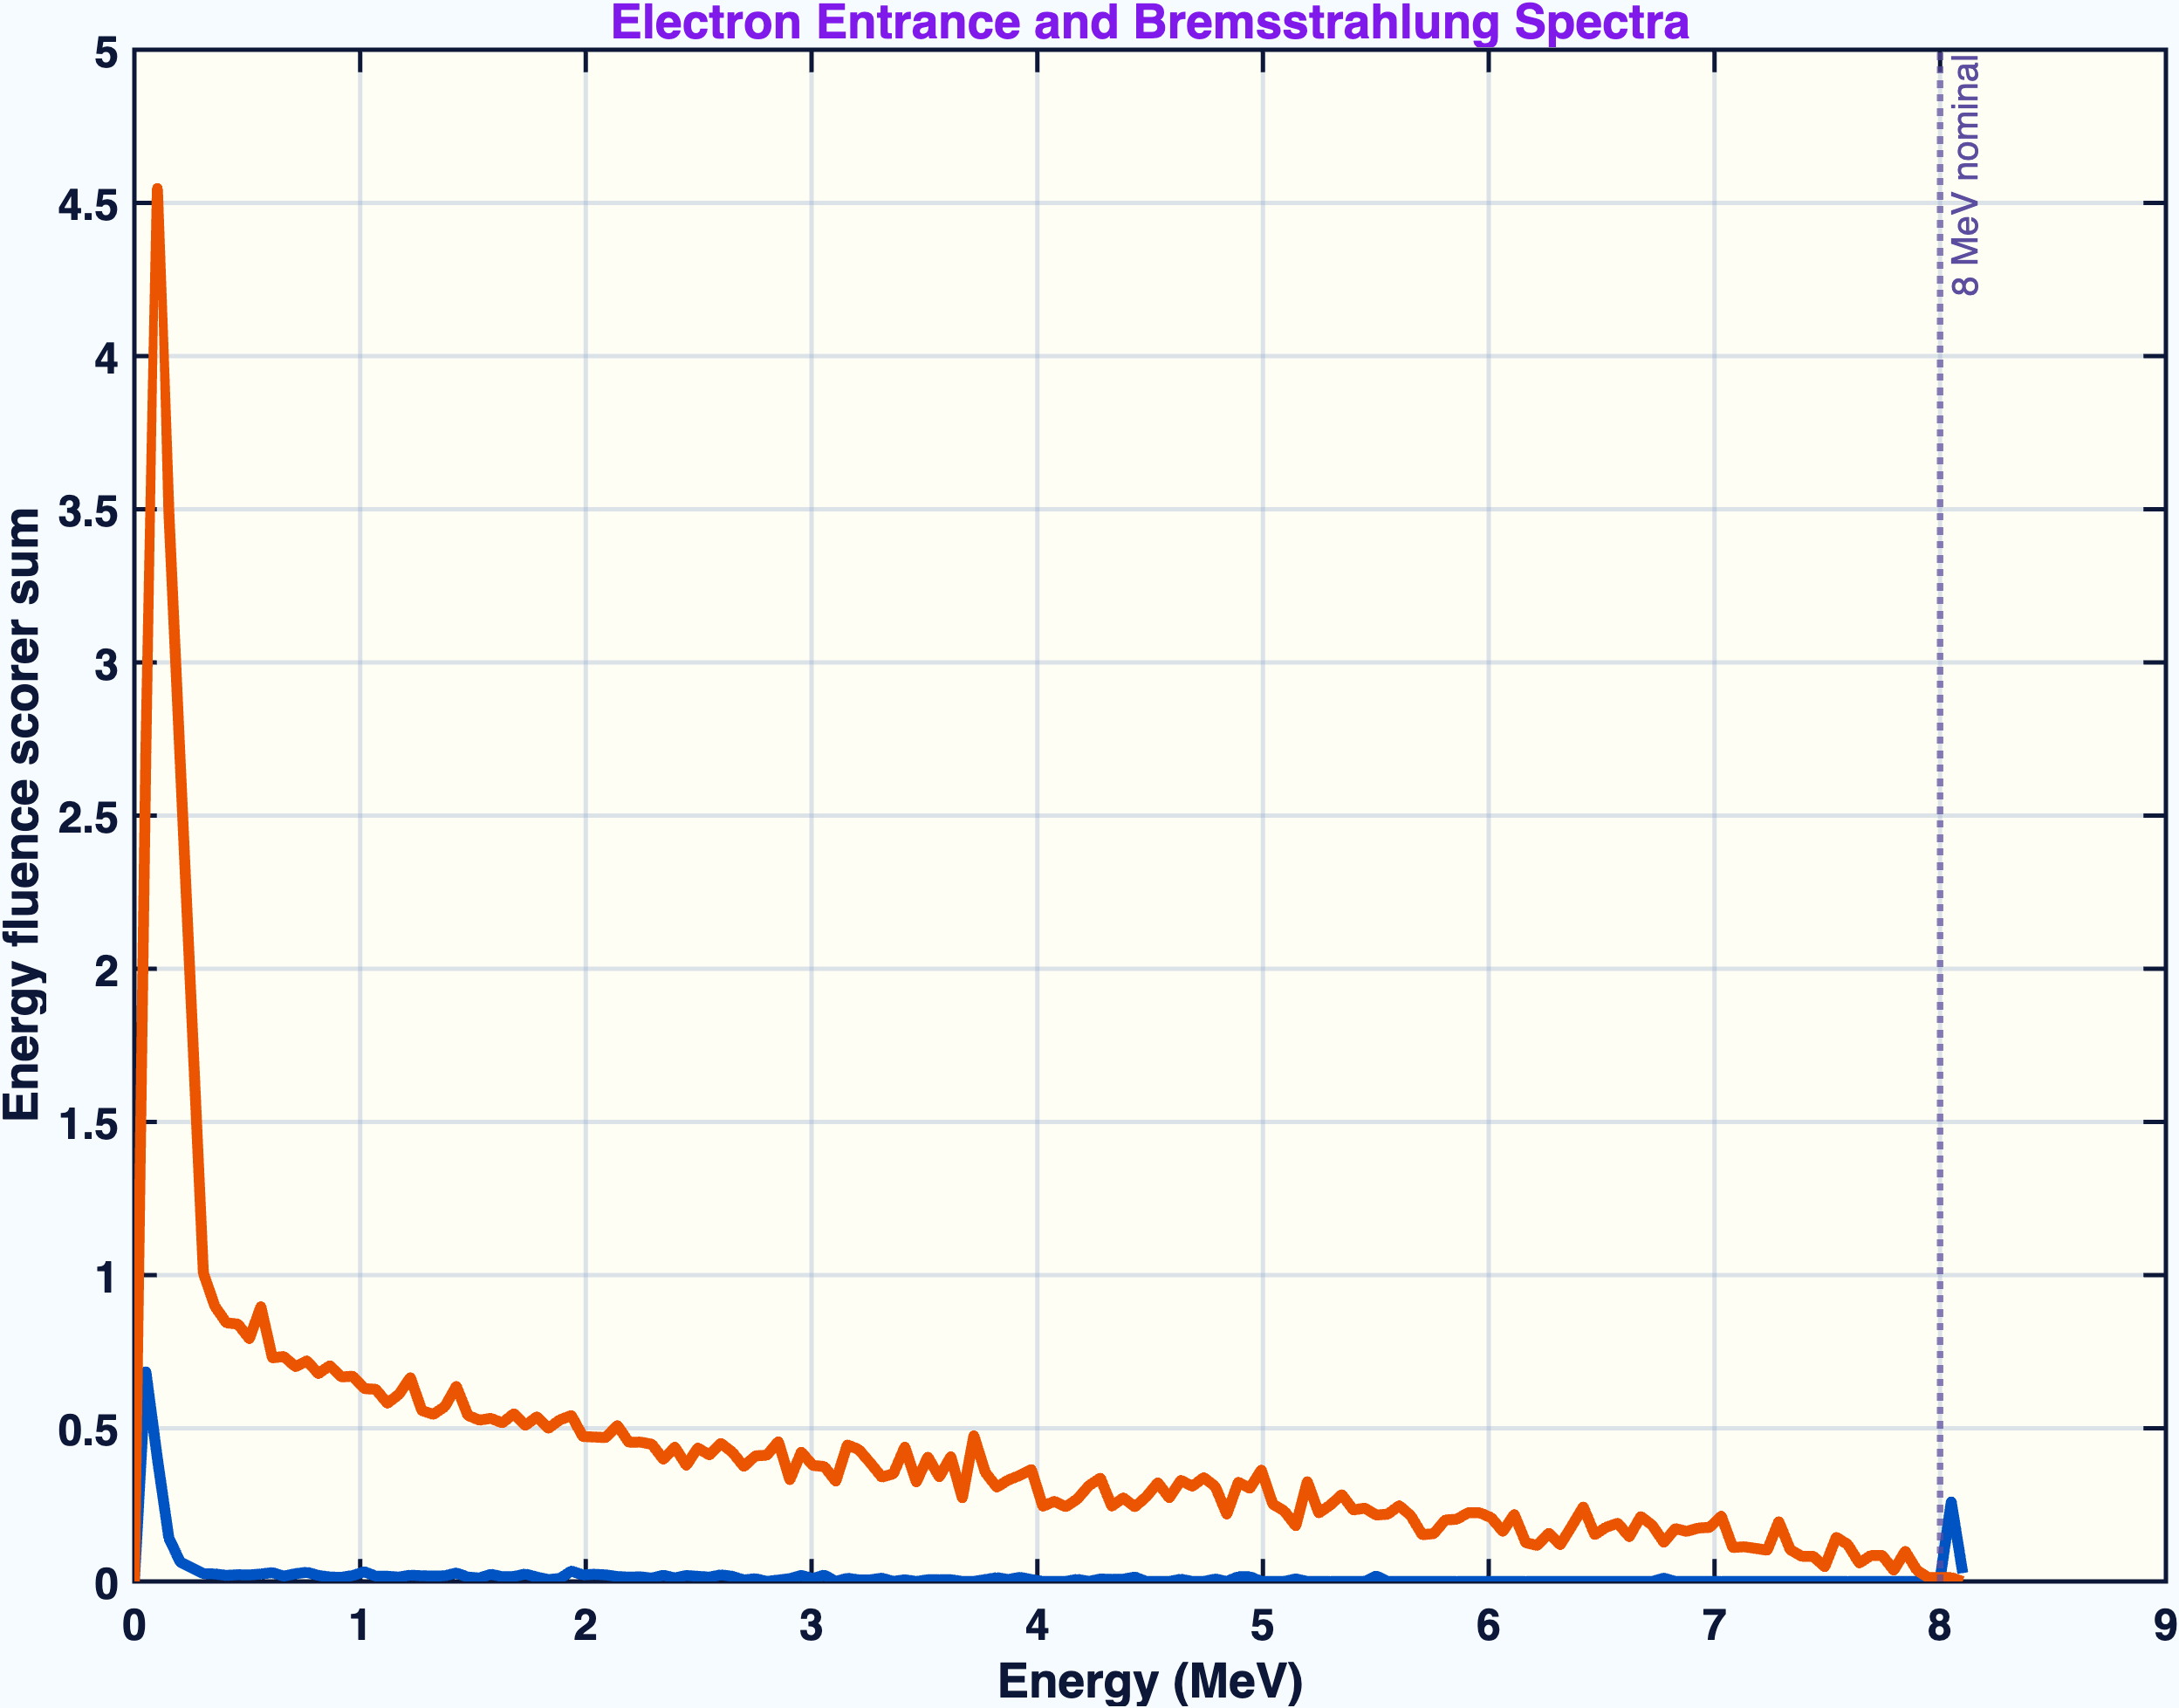
\includegraphics{./figures_matlab/pptx_deck_assets/07_energy_spectra.png}
\caption{Figure 6. Electron and photon spectral diagnostics.}
\end{figure}

\textbf{Figure 6.} Entrance electron spectrum and exit
photon/bremsstrahlung diagnostic. The plot supports the beam-transport
validation chain and provides context for secondary radiation.

\hypertarget{heat-load-1}{%
\subsection{3.7 Heat Load}\label{heat-load-1}}

The estimated cold heat load is \(0.064\,\mathrm{W}\) per active
irradiation side. The warm heat load is \(0.644\,\mathrm{W}\) per active
side. Since the target is irradiated from one side at a time, these are
not added as a simultaneous thermal load. The cold result is the most
important cryogenic feasibility number because the target material must
remain near the cold irradiation condition while radicals are produced.

\begin{figure}
\centering
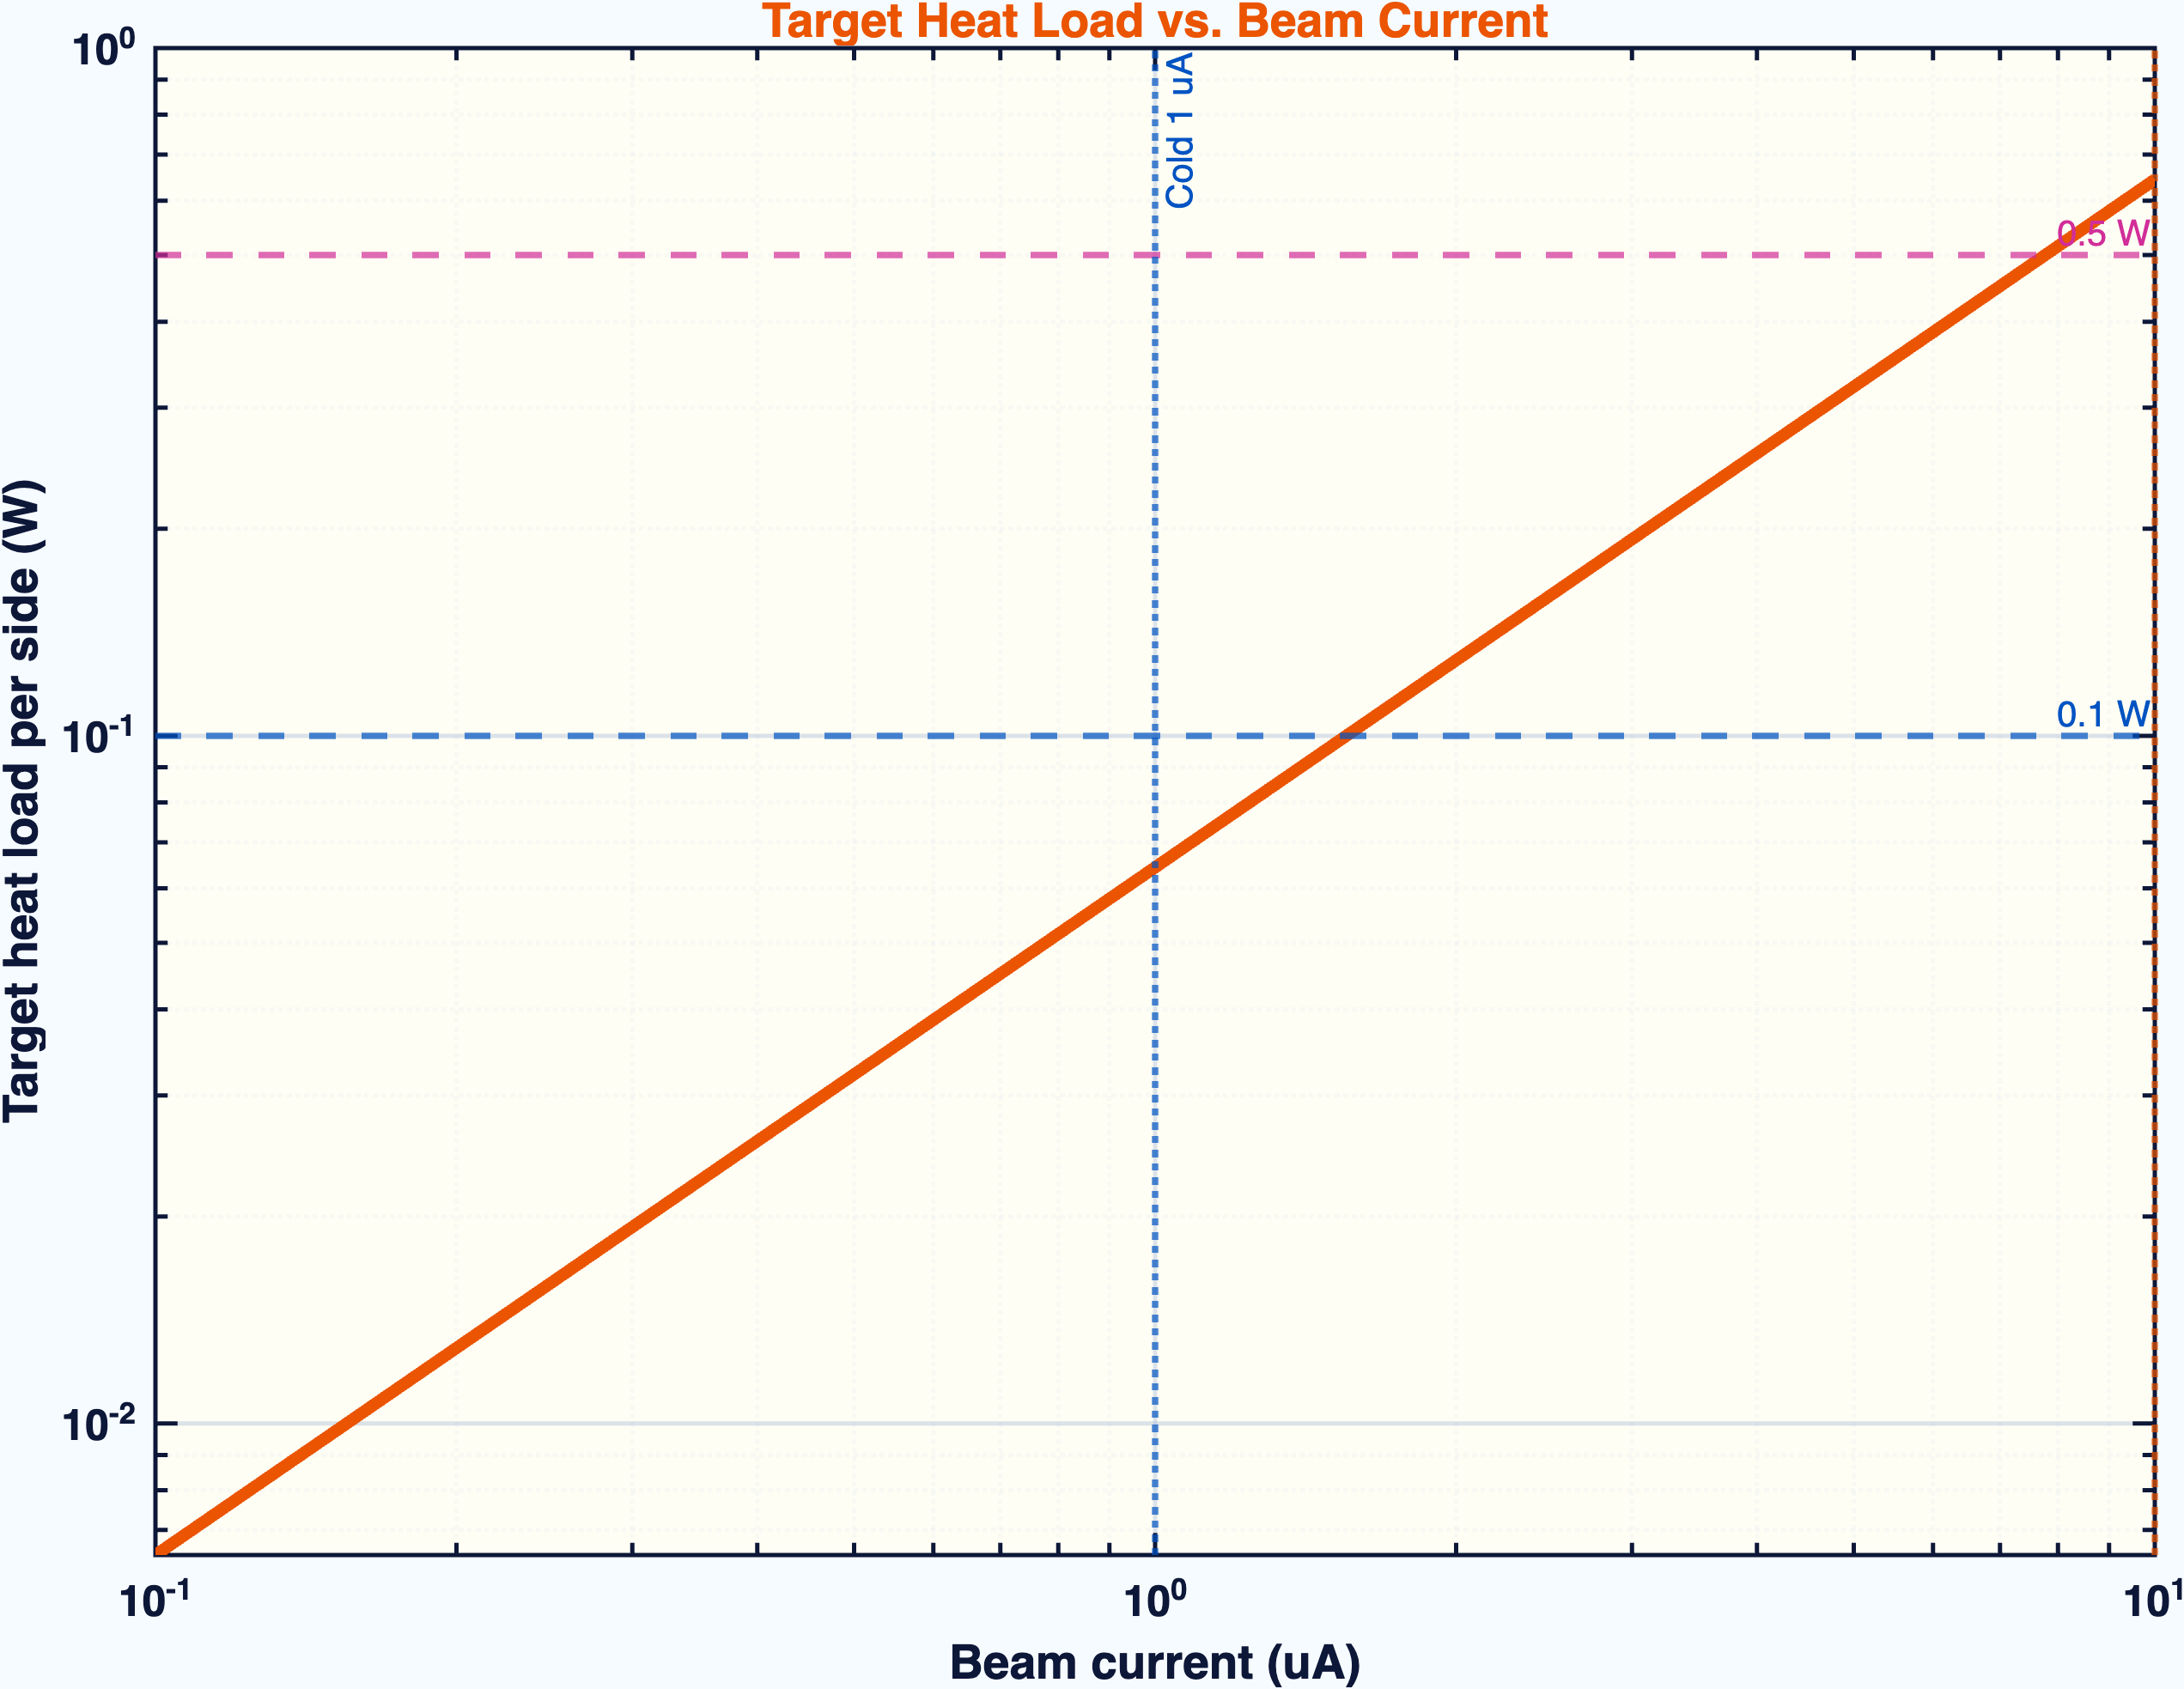
\includegraphics{./figures_matlab/pptx_deck_assets/08_heat_load_vs_current.png}
\caption{Figure 7. Target heat load versus beam current.}
\end{figure}

\textbf{Figure 7.} Target heat load versus beam current. Deposited power
is derived from total target energy deposition per primary and scaled by
electron rate. This figure is used to assess compatibility with cold
irradiation.

\hypertarget{supplemental-diagnostic-panel}{%
\subsection{3.8 Supplemental Diagnostic
Panel}\label{supplemental-diagnostic-panel}}

The supplemental multi-panel diagnostic provides an independent analysis
product from the same scorer family {[}1,2{]}. It includes dose-depth
behavior, LET-like proxy behavior, radical-yield proxy visualization,
diffusion-radius context, dose-map information, lateral uniformity,
energy spectra, bead-dose information, and current-dependent heat-load
scaling. This figure is retained as a compact record of the broader
diagnostic workflow supporting the publication figures.

\begin{figure}
\centering
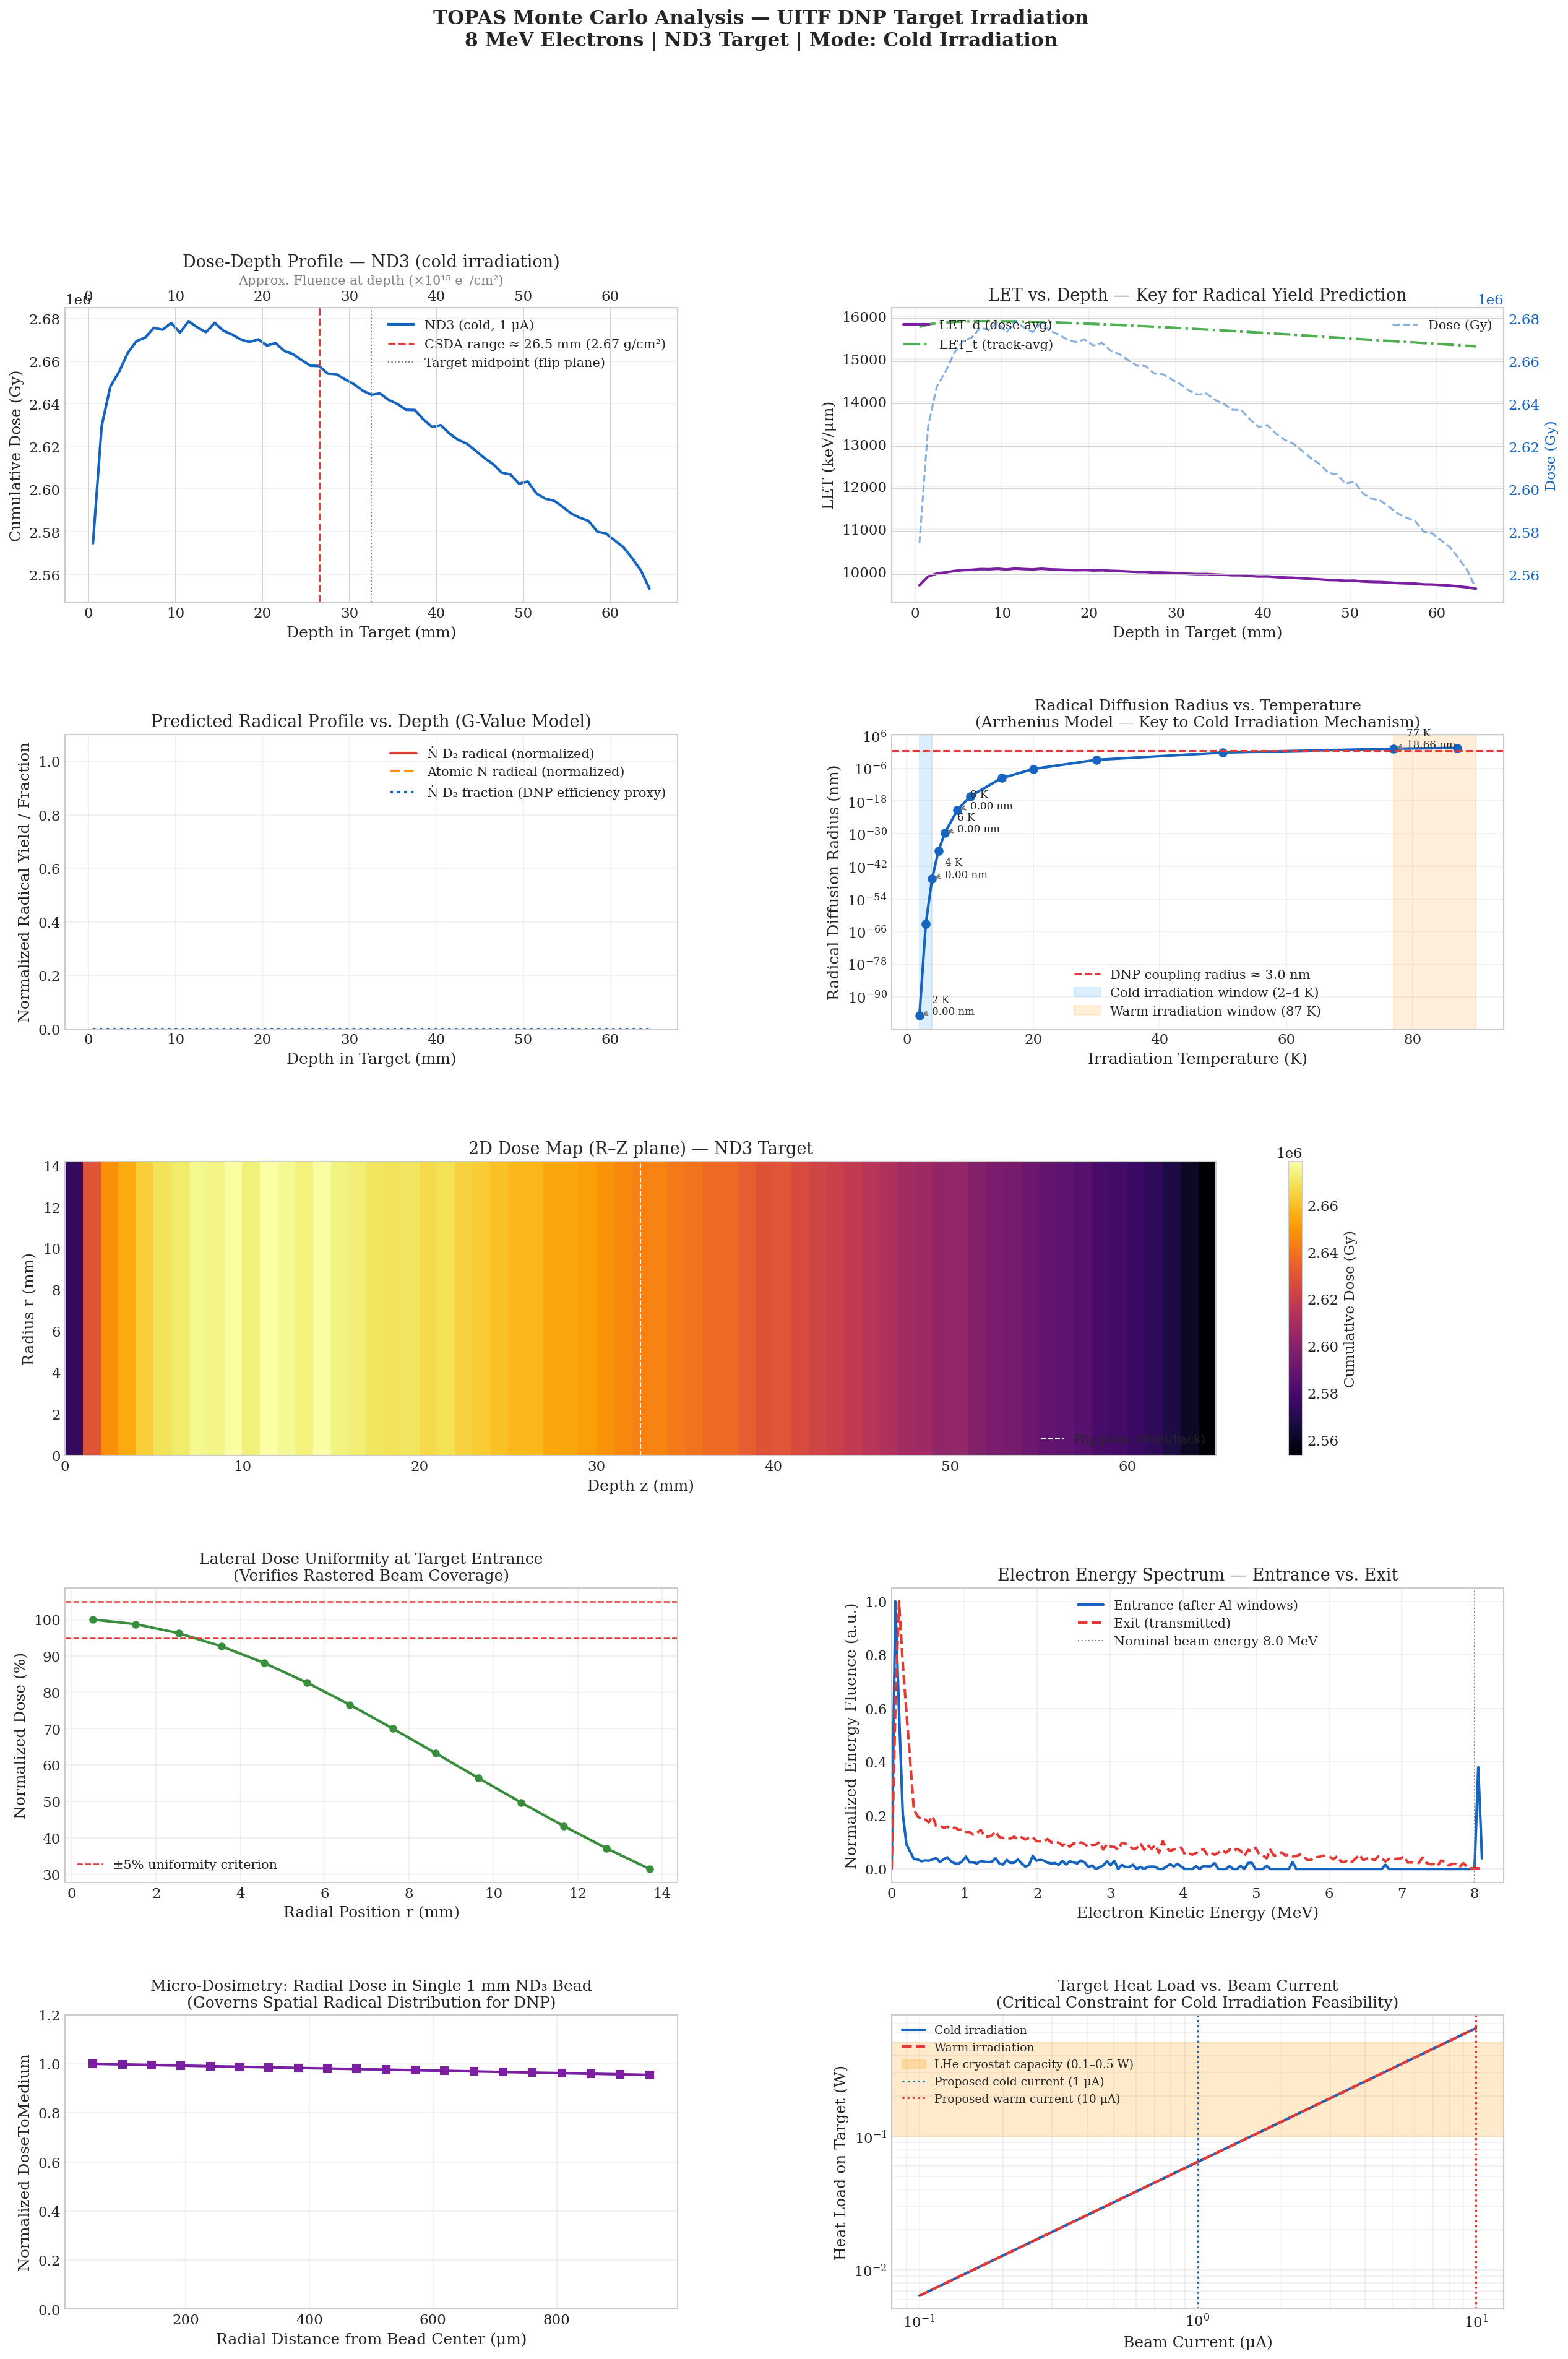
\includegraphics{./figures/DNP_UITF_Analysis_ND3_cold.png}
\caption{Figure 8. Supplemental multi-panel cold ND3 diagnostic
summary.}
\end{figure}

\textbf{Figure 8.} Supplemental multi-panel cold ND3 diagnostic summary.
The panel is useful as a compact summary of the full post-processing
workflow, including direct Monte Carlo quantities and derived
polarized-target interpretation proxies.

\hypertarget{quantitative-summary}{%
\subsection{3.9 Quantitative Summary}\label{quantitative-summary}}

\textbf{Table 1. Proposal-scaled electron fluence, mean cumulative dose,
and heat load.}

\begin{longtable}[]{@{}
  >{\raggedright\arraybackslash}p{(\columnwidth - 14\tabcolsep) * \real{0.10}}
  >{\raggedleft\arraybackslash}p{(\columnwidth - 14\tabcolsep) * \real{0.13}}
  >{\raggedleft\arraybackslash}p{(\columnwidth - 14\tabcolsep) * \real{0.13}}
  >{\raggedleft\arraybackslash}p{(\columnwidth - 14\tabcolsep) * \real{0.13}}
  >{\raggedleft\arraybackslash}p{(\columnwidth - 14\tabcolsep) * \real{0.13}}
  >{\raggedleft\arraybackslash}p{(\columnwidth - 14\tabcolsep) * \real{0.13}}
  >{\raggedleft\arraybackslash}p{(\columnwidth - 14\tabcolsep) * \real{0.13}}
  >{\raggedleft\arraybackslash}p{(\columnwidth - 14\tabcolsep) * \real{0.13}}@{}}
\toprule
Mode & Current & Proposal fluence per side & Delivered fluence per side
& Front/back total fluence & Mean dose per side & Mean front/back dose &
Heat load per active side \\
\midrule
\endhead
Cold & \(1\,\mu\mathrm{A}\) &
\(5.00 \times 10^{15}\,\mathrm{e}^{-}\,\mathrm{cm}^{-2}\) &
\(4.97 \times 10^{15}\,\mathrm{e}^{-}\,\mathrm{cm}^{-2}\) &
\(9.94 \times 10^{15}\,\mathrm{e}^{-}\,\mathrm{cm}^{-2}\) &
\(1.32 \times 10^{6}\,\mathrm{Gy}\) &
\(2.63 \times 10^{6}\,\mathrm{Gy}\) & \(0.064\,\mathrm{W}\) \\
Warm & \(10\,\mu\mathrm{A}\) &
\(1.00 \times 10^{17}\,\mathrm{e}^{-}\,\mathrm{cm}^{-2}\) &
\(9.97 \times 10^{16}\,\mathrm{e}^{-}\,\mathrm{cm}^{-2}\) &
\(1.99 \times 10^{17}\,\mathrm{e}^{-}\,\mathrm{cm}^{-2}\) &
\(2.64 \times 10^{7}\,\mathrm{Gy}\) &
\(5.29 \times 10^{7}\,\mathrm{Gy}\) & \(0.644\,\mathrm{W}\) \\
\bottomrule
\end{longtable}

The cold delivered fluence is within approximately one percent of the
target value, and the warm delivered fluence is within approximately one
percent of the target value. This validates the current-time-fluence
scaling used for the proposal operating points.

\hypertarget{discussion}{%
\section{4. Discussion}\label{discussion}}

The central result is that the target geometry cannot be interpreted
using a one-sided \(8\,\mathrm{MeV}\) irradiation alone. The front/back
protocol is required by electron range and energy-loss physics. This is
directly relevant to polarized target preparation because the useful
material property is not the dose at a single face, but the retained
radical population across the target batch.

The calculation also separates irradiation quality from
material-response interpretation. Dose and fluence establish where
ionization energy is delivered. LET-like proxies provide limited
track-structure context. However, the final paramagnetic-center
population depends on radical formation, radical survival,
recombination, temperature, annealing, and crystal-state effects. These
are not computed directly by TOPAS. Electron spin resonance, NMR-based
polarization measurements, or direct post-irradiation polarization tests
are required before the simulation can be converted into a claim about
final DNP performance {[}4-6{]}.

The cold heat-load result is promising as a feasibility indicator. A
deposited power of \(0.064\,\mathrm{W}\) per active side is within the
scale where low-temperature operation may be plausible, subject to the
actual refrigerator, thermal coupling, target holder, and beam
structure. The warm heat load is larger but belongs to a different
thermal environment and should be interpreted separately.

\hypertarget{model-scope-and-experimental-benchmarks}{%
\subsection{4.1 Model Scope and Experimental
Benchmarks}\label{model-scope-and-experimental-benchmarks}}

The present calculation is best interpreted as a feasibility and
beam-transport study for the proposed irradiation geometry. It
establishes the dose, fluence, target-volume coverage, spectral
diagnostics, and heat-load scale needed to evaluate the irradiation
protocol, while leaving the final material-response observables to
dedicated experimental benchmarks.

The packed ND3 target is represented as a batch-averaged mass
distribution over the holder volume. This treatment is appropriate for
proposal-scale fluence and heat-load normalization, and it preserves the
relevant target mass for the reported dose estimates. A resolved
bead-packing model would be a useful extension if bead-to-bead dose
variation becomes a design driver. Similarly, the cryostat and holder
are represented by physics-motivated proxy dimensions and should be
updated as engineering drawings mature; this refinement would improve
geometry fidelity without changing the central range-based conclusion
that one-sided \(8\,\mathrm{MeV}\) exposure is insufficient over the
full target length.

The LET-like and radical-yield proxy panels are used as diagnostic
context for where ionization energy is deposited. They are not treated
as direct predictions of radical species, radical survival, or electron
chemical effectiveness. The simulation therefore motivates, rather than
replaces, the experimental benchmarks most relevant to DNP material
quality: ESR characterization of the irradiated radical population and
NMR or polarization measurements after the proposed irradiation and
thermal history.

For reproducibility, the tabulated values should remain tied to the
archived production outputs and analysis-script version used for the
final manuscript, so that each reported number can be traced to a single
analysis provenance chain.

\hypertarget{conclusion}{%
\section{5. Conclusion}\label{conclusion}}

The Monte Carlo model supports the feasibility of a two-sided
\(8\,\mathrm{MeV}\) electron irradiation protocol for cryogenic packed
ND3 polarized-target preparation. The front-only dose field is
range-limited over the \(6.5\,\mathrm{cm}\) target length, making
back-side irradiation necessary for proposal-relevant target-volume
coverage. The front/back cumulative dose field, electron fluence
scaling, radial coverage, spectral checks, and heat-load estimate form a
coherent validation chain for the irradiation concept.

For the cold \(1\,\mu\mathrm{A}\) case, the model delivers
\(4.97 \times 10^{15}\,\mathrm{e}^{-}\,\mathrm{cm}^{-2}\) per side and
estimates \(0.064\,\mathrm{W}\) target heat load per active side. For
the warm \(10\,\mu\mathrm{A}\) case, the model delivers
\(9.97 \times 10^{16}\,\mathrm{e}^{-}\,\mathrm{cm}^{-2}\) per side and
estimates \(0.644\,\mathrm{W}\) per active side. These results support
continued development of the irradiation protocol, with the key caveat
that radical chemistry and final DNP polarization must be validated
experimentally.

\hypertarget{acknowledgments}{%
\section{Acknowledgments}\label{acknowledgments}}

This manuscript was prepared by Samuel Takwirira for the UNH DNP Group /
Jefferson Lab Target Group collaboration. The author gratefully
acknowledges Dr.~Karl Slifer for guidance during critique sessions that
helped steer the work toward its intended direction. The work is
motivated by polarized fixed-target material preparation and by the
broader literature on irradiated ammonia targets for DNP {[}3-6{]}.

\hypertarget{data-and-code-availability}{%
\section{Data and Code Availability}\label{data-and-code-availability}}

The TOPAS simulation inputs, analysis scripts, scorer outputs, and
figure-generation materials used in this work are archived in the
project repository: https://github.com/SamuelBarachel/UITF02. The
numerical values reported in the tables and figures were generated from
the archived production outputs associated with this manuscript.
Additional project materials may be made available by the author upon
reasonable request, subject to collaboration and institutional
constraints.

\hypertarget{references}{%
\section{References}\label{references}}

{[}1{]} S. Agostinelli et al., ``GEANT4 - A simulation toolkit,''
\emph{Nuclear Instruments and Methods in Physics Research Section A},
vol.~506, no. 3, pp.~250-303, 2003. doi:
10.1016/S0168-9002(03)01368-8.\\
{[}2{]} J. Perl, J. Shin, J. Schumann, B. Faddegon, and H. Paganetti,
``TOPAS: An innovative proton Monte Carlo platform for research and
clinical applications,'' \emph{Medical Physics}, vol.~39, no. 11,
pp.~6818-6837, 2012. doi: 10.1118/1.4758060.\\
{[}3{]} D. G. Crabb and W. Meyer, ``Solid polarized targets for nuclear
and particle physics experiments,'' \emph{Annual Review of Nuclear and
Particle Science}, vol.~47, pp.~67-109, 1997. doi:
10.1146/annurev.nucl.47.1.67.\\
{[}4{]} W. Meyer, ``Ammonia as a polarized solid target material - a
review,'' \emph{Nuclear Instruments and Methods in Physics Research
Section A}, vol.~526, issues 1-2, pp.~12-21, 2004. doi:
10.1016/j.nima.2004.03.145.\\
{[}5{]} W. Meyer, K. H. Althoff, W. Havenith, and W. Thiel, ``Dynamic
deuteron polarization in irradiated D-ammonia (ND3) and its first use in
a high energy photon beam,'' \emph{Nuclear Instruments and Methods in
Physics Research Section A}, vol.~227, no. 1, pp.~35-44, 1984. doi:
10.1016/0168-9002(84)90098-6.\\
{[}6{]} A. Conover, V. Y. S. Bandara, D. Keller, and F. Bateman, ``Bulk
irradiation of ammonia for polarized target experiments,'' \emph{Nuclear
Instruments and Methods in Physics Research Section A}, vol.~1068,
article 169717, 2024. doi: 10.1016/j.nima.2024.169717.\\
{[}7{]} UNH-UITF BeamNetUS Proposal, internal project document.

\end{document}
